% Options for packages loaded elsewhere
% Options for packages loaded elsewhere
\PassOptionsToPackage{unicode}{hyperref}
\PassOptionsToPackage{hyphens}{url}
\PassOptionsToPackage{dvipsnames,svgnames,x11names}{xcolor}
%
\documentclass[
  portuguese,
  letterpaper,
  DIV=11,
  numbers=noendperiod]{scrreprt}
\usepackage{xcolor}
\usepackage{amsmath,amssymb}
\setcounter{secnumdepth}{5}
\usepackage{iftex}
\ifPDFTeX
  \usepackage[T1]{fontenc}
  \usepackage[utf8]{inputenc}
  \usepackage{textcomp} % provide euro and other symbols
\else % if luatex or xetex
  \usepackage{unicode-math} % this also loads fontspec
  \defaultfontfeatures{Scale=MatchLowercase}
  \defaultfontfeatures[\rmfamily]{Ligatures=TeX,Scale=1}
\fi
\usepackage{lmodern}
\ifPDFTeX\else
  % xetex/luatex font selection
\fi
% Use upquote if available, for straight quotes in verbatim environments
\IfFileExists{upquote.sty}{\usepackage{upquote}}{}
\IfFileExists{microtype.sty}{% use microtype if available
  \usepackage[]{microtype}
  \UseMicrotypeSet[protrusion]{basicmath} % disable protrusion for tt fonts
}{}
\makeatletter
\@ifundefined{KOMAClassName}{% if non-KOMA class
  \IfFileExists{parskip.sty}{%
    \usepackage{parskip}
  }{% else
    \setlength{\parindent}{0pt}
    \setlength{\parskip}{6pt plus 2pt minus 1pt}}
}{% if KOMA class
  \KOMAoptions{parskip=half}}
\makeatother
% Make \paragraph and \subparagraph free-standing
\makeatletter
\ifx\paragraph\undefined\else
  \let\oldparagraph\paragraph
  \renewcommand{\paragraph}{
    \@ifstar
      \xxxParagraphStar
      \xxxParagraphNoStar
  }
  \newcommand{\xxxParagraphStar}[1]{\oldparagraph*{#1}\mbox{}}
  \newcommand{\xxxParagraphNoStar}[1]{\oldparagraph{#1}\mbox{}}
\fi
\ifx\subparagraph\undefined\else
  \let\oldsubparagraph\subparagraph
  \renewcommand{\subparagraph}{
    \@ifstar
      \xxxSubParagraphStar
      \xxxSubParagraphNoStar
  }
  \newcommand{\xxxSubParagraphStar}[1]{\oldsubparagraph*{#1}\mbox{}}
  \newcommand{\xxxSubParagraphNoStar}[1]{\oldsubparagraph{#1}\mbox{}}
\fi
\makeatother

\usepackage{color}
\usepackage{fancyvrb}
\newcommand{\VerbBar}{|}
\newcommand{\VERB}{\Verb[commandchars=\\\{\}]}
\DefineVerbatimEnvironment{Highlighting}{Verbatim}{commandchars=\\\{\}}
% Add ',fontsize=\small' for more characters per line
\usepackage{framed}
\definecolor{shadecolor}{RGB}{241,243,245}
\newenvironment{Shaded}{\begin{snugshade}}{\end{snugshade}}
\newcommand{\AlertTok}[1]{\textcolor[rgb]{0.68,0.00,0.00}{#1}}
\newcommand{\AnnotationTok}[1]{\textcolor[rgb]{0.37,0.37,0.37}{#1}}
\newcommand{\AttributeTok}[1]{\textcolor[rgb]{0.40,0.45,0.13}{#1}}
\newcommand{\BaseNTok}[1]{\textcolor[rgb]{0.68,0.00,0.00}{#1}}
\newcommand{\BuiltInTok}[1]{\textcolor[rgb]{0.00,0.23,0.31}{#1}}
\newcommand{\CharTok}[1]{\textcolor[rgb]{0.13,0.47,0.30}{#1}}
\newcommand{\CommentTok}[1]{\textcolor[rgb]{0.37,0.37,0.37}{#1}}
\newcommand{\CommentVarTok}[1]{\textcolor[rgb]{0.37,0.37,0.37}{\textit{#1}}}
\newcommand{\ConstantTok}[1]{\textcolor[rgb]{0.56,0.35,0.01}{#1}}
\newcommand{\ControlFlowTok}[1]{\textcolor[rgb]{0.00,0.23,0.31}{\textbf{#1}}}
\newcommand{\DataTypeTok}[1]{\textcolor[rgb]{0.68,0.00,0.00}{#1}}
\newcommand{\DecValTok}[1]{\textcolor[rgb]{0.68,0.00,0.00}{#1}}
\newcommand{\DocumentationTok}[1]{\textcolor[rgb]{0.37,0.37,0.37}{\textit{#1}}}
\newcommand{\ErrorTok}[1]{\textcolor[rgb]{0.68,0.00,0.00}{#1}}
\newcommand{\ExtensionTok}[1]{\textcolor[rgb]{0.00,0.23,0.31}{#1}}
\newcommand{\FloatTok}[1]{\textcolor[rgb]{0.68,0.00,0.00}{#1}}
\newcommand{\FunctionTok}[1]{\textcolor[rgb]{0.28,0.35,0.67}{#1}}
\newcommand{\ImportTok}[1]{\textcolor[rgb]{0.00,0.46,0.62}{#1}}
\newcommand{\InformationTok}[1]{\textcolor[rgb]{0.37,0.37,0.37}{#1}}
\newcommand{\KeywordTok}[1]{\textcolor[rgb]{0.00,0.23,0.31}{\textbf{#1}}}
\newcommand{\NormalTok}[1]{\textcolor[rgb]{0.00,0.23,0.31}{#1}}
\newcommand{\OperatorTok}[1]{\textcolor[rgb]{0.37,0.37,0.37}{#1}}
\newcommand{\OtherTok}[1]{\textcolor[rgb]{0.00,0.23,0.31}{#1}}
\newcommand{\PreprocessorTok}[1]{\textcolor[rgb]{0.68,0.00,0.00}{#1}}
\newcommand{\RegionMarkerTok}[1]{\textcolor[rgb]{0.00,0.23,0.31}{#1}}
\newcommand{\SpecialCharTok}[1]{\textcolor[rgb]{0.37,0.37,0.37}{#1}}
\newcommand{\SpecialStringTok}[1]{\textcolor[rgb]{0.13,0.47,0.30}{#1}}
\newcommand{\StringTok}[1]{\textcolor[rgb]{0.13,0.47,0.30}{#1}}
\newcommand{\VariableTok}[1]{\textcolor[rgb]{0.07,0.07,0.07}{#1}}
\newcommand{\VerbatimStringTok}[1]{\textcolor[rgb]{0.13,0.47,0.30}{#1}}
\newcommand{\WarningTok}[1]{\textcolor[rgb]{0.37,0.37,0.37}{\textit{#1}}}

\usepackage{longtable,booktabs,array}
\usepackage{calc} % for calculating minipage widths
% Correct order of tables after \paragraph or \subparagraph
\usepackage{etoolbox}
\makeatletter
\patchcmd\longtable{\par}{\if@noskipsec\mbox{}\fi\par}{}{}
\makeatother
% Allow footnotes in longtable head/foot
\IfFileExists{footnotehyper.sty}{\usepackage{footnotehyper}}{\usepackage{footnote}}
\makesavenoteenv{longtable}
\usepackage{graphicx}
\makeatletter
\newsavebox\pandoc@box
\newcommand*\pandocbounded[1]{% scales image to fit in text height/width
  \sbox\pandoc@box{#1}%
  \Gscale@div\@tempa{\textheight}{\dimexpr\ht\pandoc@box+\dp\pandoc@box\relax}%
  \Gscale@div\@tempb{\linewidth}{\wd\pandoc@box}%
  \ifdim\@tempb\p@<\@tempa\p@\let\@tempa\@tempb\fi% select the smaller of both
  \ifdim\@tempa\p@<\p@\scalebox{\@tempa}{\usebox\pandoc@box}%
  \else\usebox{\pandoc@box}%
  \fi%
}
% Set default figure placement to htbp
\def\fps@figure{htbp}
\makeatother



\ifLuaTeX
\usepackage[bidi=basic]{babel}
\else
\usepackage[bidi=default]{babel}
\fi
% get rid of language-specific shorthands (see #6817):
\let\LanguageShortHands\languageshorthands
\def\languageshorthands#1{}


\setlength{\emergencystretch}{3em} % prevent overfull lines

\providecommand{\tightlist}{%
  \setlength{\itemsep}{0pt}\setlength{\parskip}{0pt}}



 


<style>
   /* ===== largura máxima do conteúdo ===== */
  :root { --content-max-width: 1600px; }

  /* ===== cores utilitárias (suas classes) ===== */
  .red  { color: #e53935; }
  .blue { color: dodgerblue; }
  .darkblue  { color: #003366; }   /* azul escuro */
  .darkgreen { color: #006400; }   /* verde escuro */
  .orange    { color: #ff8c00; }   /* laranja */
  .purple    { color: #800080; }   /* roxo */
  .note { color:#6f42c1; background:#f3e8ff; padding:2px 6px; border-radius:6px; }

  /* ===== BOTÃO CENTRAL personalizável ===== */
  #qst-centered {
    position: fixed;
    top: 12px;
    left: 50%;
    transform: translateX(-50%);
    z-index: 1031;
    display: inline-flex;
    align-items: center;
    justify-content: center;
    width: 36px;
    height: 36px;
    border-radius: 999px;
    background: #fff;
    border: 1px solid #e6ecf3;
    box-shadow: 0 2px 8px rgba(0,0,0,.08);
    cursor: pointer;
  }
  #qst-centered:hover {
    box-shadow: 0 3px 12px rgba(0,0,0,.12);
    border-color: #d8e2ef;
  }
  #qst-centered .qst-bar {
    width: 18px; height: 2px; background:#333; margin: 2px 0;
  }

  /* Em telas pequenas, deixe o comportamento padrão do tema */
  @media (max-width: 991.98px){
    #qst-centered { display: none; }
  }

  /* Evitar que o botão sobreponha o H1 ao navegar por âncoras */
  .content h1.title, .content h1 { scroll-margin-top: 60px; }
</style>



<script>
  document.addEventListener('DOMContentLoaded', function () {
    // 1) Verifique se o include carregou: deve haver o quadradinho verde no canto (body::after)
    // 2) Criar um botão central próprio (independente do botão do tema)
    if (!document.getElementById('qst-centered')) {
      const b = document.createElement('button');
      b.id = 'qst-centered';
      b.setAttribute('type','button');
      b.setAttribute('title','Mostrar/ocultar barra lateral');

      for (let i=0;i<3;i++){
        const bar = document.createElement('div');
        bar.className = 'qst-bar';
        b.appendChild(bar);
      }
      document.body.appendChild(b);

      // Handler do clique: alterna o estado do sidebar usando Bootstrap Collapse
      b.addEventListener('click', () => {
        try {
          const sidebar = document.querySelector('#quarto-sidebar');
          const body = document.body;

          // alterna uma classe no body (útil para temas que usam isso)
          body.classList.toggle('sidebar-collapsed');

          if (sidebar) {
            // se estiver colapsado, mostramos; se estiver aberto, escondemos
            const isOpen = sidebar.classList.contains('show');
            // tenta usar a API do Bootstrap, se estiver presente
            const bs = (window.bootstrap && window.bootstrap.Collapse)
              ? window.bootstrap.Collapse.getOrCreateInstance(sidebar)
              : null;

            if (bs) {
              if (isOpen) { bs.hide(); } else { bs.show(); }
            } else {
              // fallback: alterna class "show" manualmente
              sidebar.classList.toggle('show');
            }

            // mantém a classe do body coerente
            if (sidebar.classList.contains('show')) {
              body.classList.remove('sidebar-collapsed');
            } else {
              body.classList.add('sidebar-collapsed');
            }
          }
        } catch (e) {
          console.warn('Toggle central falhou:', e);
        }
      });
    }
  });
</script>
<script>
  (function(){
    function pickVisible(el){ return el && el.offsetParent !== null; }

    function findNativeToggle(){
      // 1) seletores “clássicos” do Quarto (cobrindo variações)
      const sels = [
        '#quarto-sidebar-toggle',
        '.quarto-sidebar-toggle',
        'button.sidebar-toggle',
        'button[aria-controls="quarto-sidebar"]',
        'a[aria-controls="quarto-sidebar"]',
        '[data-bs-target="#quarto-sidebar"]',
        '[aria-label*="sidebar" i]'
      ];
      for (const s of sels){
        const el = document.querySelector(s);
        if (pickVisible(el)) return el;
      }

      // 2) Heurística: procura um botão pequeno no canto sup. esquerdo
      const candidates = Array.from(document.querySelectorAll('button, a, .btn'));
      const ranked = candidates
        .map(el => [el, el.getBoundingClientRect()])
        .filter(([el, r]) => r.width > 20 && r.width < 64 && r.height > 20 && r.height < 64 && r.top >= 0 && r.top < 120 && r.left >= 0 && r.left < 140)
        .sort((a,b) => (a[1].top - b[1].top) || (a[1].left - b[1].left));
      return ranked.length ? ranked[0][0] : null;
    }

    function moveNativeToggle(){
      const btn = findNativeToggle();
      if (!btn) return;

      // reposiciona o PRÓPRIO botão nativo
      btn.style.position   = 'fixed';
      btn.style.left       = '50%';
      btn.style.top        = '12px';
      btn.style.transform  = 'translateX(-50%)';
      btn.style.zIndex     = '1060';

      // estética opcional (remova se quiser o padrão do tema)
      btn.style.background = '#fff';
      btn.style.border     = '1px solid #e6ecf3';
      btn.style.boxShadow  = '0 2px 8px rgba(0,0,0,.08)';
      btn.style.borderRadius = '999px';
      btn.style.width      = '36px';
      btn.style.height     = '36px';
      btn.style.display    = 'inline-flex';
      btn.style.alignItems = 'center';
      btn.style.justifyContent = 'center';
      btn.style.padding    = '0';
    }

    function wire(){
      moveNativeToggle();
      // se o DOM mudar (p.ex. render tardio), tentamos de novo
      const obs = new MutationObserver(() => moveNativeToggle());
      obs.observe(document.body, {childList:true, subtree:true});
      // também ao redimensionar
      window.addEventListener('resize', moveNativeToggle);
    }

    if (document.readyState === 'loading'){
      document.addEventListener('DOMContentLoaded', wire);
    } else {
      wire();
    }
  })();
</script>

<style>
  /* Esconde o botão nativo original no canto ESQUERDO em telas médias+,
     caso ele reapareça por algum motivo (opcional). */
  @media (min-width: 992px){
    .sidebar .quarto-sidebar-toggle,
    .sidebar #quarto-sidebar-toggle,
    .sidebar button.sidebar-toggle{ visibility:hidden !important; }
  }
  /* Em telas pequenas, deixe como está (botão no canto esq.) */
  @media (max-width: 991.98px){
    /* nada aqui: usamos o padrão do tema */
  }
</style>
<style>
  /* ===== LARGURA MENOR PARA SIDEBAR E TOC =====
     Aplica só em telas médias/grandes para não atrapalhar mobile */
  @media (min-width: 992px){

    /* (1) Se o seu Quarto expõe variáveis, use-as (fica mais limpo) */
    :root{
      --sidebar-width: 220px;            /* esquerda */
      --margin-sidebar-width: 240px;     /* TOC à direita */
    }

    /* (2) Fallback robusto (quando tema/versão não usa as variáveis) */
    #quarto-sidebar{
      width: var(--sidebar-width) !important;
    }
    /* alguns temas têm contêiner interno com largura própria */
    #quarto-sidebar .sidebar,
    #quarto-sidebar .sidebar-content,
    .sidebar.sidebar-navigation{
      width: var(--sidebar-width) !important;
      max-width: var(--sidebar-width) !important;
    }

    /* TOC / margin sidebar (direita) */
    #quarto-margin-sidebar{
      width: var(--margin-sidebar-width) !important;
    }
    .margin-sidebar{
      width: var(--margin-sidebar-width) !important;
      max-width: var(--margin-sidebar-width) !important;
    }

    /* (3) Diminui o espaço entre as 3 colunas (sidebar | conteúdo | TOC) */
    #quarto-content.page-columns{
      column-gap: 14px !important;  /* experimente 10–18px */
    }

    /* (4) Conteúdo central sem “colchões” extras */
    main.content{
      padding-left: 0 !important;
      padding-right: 0 !important;
    }

    /* (5) Só estética: o search acompanha a nova largura */
    #quarto-sidebar input.sidebar-search{
      width: 100% !important;
    }
  }
</style>
<style>
  /* ===== Preenche melhor a área central ===== */
  @media (min-width: 992px){

    /* use os mesmos valores que você já está usando
       para sidebar e TOC (ou deixe estes) */
    :root{
      --sidebar-width: 220px;
      --margin-sidebar-width: 240px;
    }

    /* gap entre colunas + “almofada” lateral de página (gutters) */
    :root{
      --lv-gap: 14px;       /* mesmo column-gap que você definiu */
      --lv-page-pad: 12px;  /* gutters externos (um de cada lado) */
    }

    /* Faz o track do conteúdo central ocupar todo o restante da tela */
    :root{
      --content-max-width: calc(
        100vw
        - var(--sidebar-width)
        - var(--margin-sidebar-width)
        - (2 * var(--lv-gap))
        - (2 * var(--lv-page-pad))
      ) !important;
    }

    /* Garante que o elemento não imponha um max-width menor */
    main.content{
      max-width: none !important;
      padding-left: 0 !important;
      padding-right: 0 !important;
    }

    /* Ajusta o espaçamento entre as 3 colunas */
    #quarto-content.page-columns{
      column-gap: var(--lv-gap) !important;
    }

    /* Opcional: controla os gutters externos (margens da página) */
    .page-columns{
      padding-left: var(--lv-page-pad) !important;
      padding-right: var(--lv-page-pad) !important;
    }
  }
</style>

<style>
  /* ===== Ajuste seguro de larguras sem redesenhar o grid ===== */
  @media (min-width: 992px){
    /* 1) larguras das colunas do Quarto */
    :root{
      /* sidebar (esquerda) e TOC (direita) */
      --sidebar-width:           220px;  /* ajuste aqui, ex: 200-240 */
      --margin-sidebar-width:    240px;  /* TOC; ajuste aqui, ex: 220-260 */

      /* largura máxima do conteúdo (miolo) — pode ser grande */
      --content-max-width:       2000px; /* evita “miolo” estreito */
    }

    /* 2) aplica os valores sem mexer no grid */
    #quarto-sidebar{
      width: var(--sidebar-width) !important;
      min-width: var(--sidebar-width) !important;
    }
    #quarto-margin-sidebar{
      width: var(--margin-sidebar-width) !important;
      min-width: var(--margin-sidebar-width) !important;
    }

    /* 3) respiro e liberação de largura no conteúdo */
    main.content{
      max-width: none !important;          /* ignora limites herdados */
      padding-left:  14px !important;      /* “respiro” interno */
      padding-right: 14px !important;
      overflow: visible !important;        /* não corta texto nas bordas */
      box-sizing: border-box !important;
    }

    /* 4) diminui o espaço entre colunas (sem trocar ordem) */
    #quarto-content.page-columns{
      column-gap: 14px !important;         /* ajuste: 10–16px */
    }
  }

  /* Em telas pequenas, deixa o padrão móvel */
  @media (max-width: 991.98px){
    main.content{
      padding-left: 12px !important;
      padding-right: 12px !important;
    }
  }
</style>
<style>
  /* ===== Correções para telas pequenas (celular) ===== */
  @media (max-width: 991.98px){

    /* 1) Some com o TOC direito para liberar largura */
    #quarto-margin-sidebar{
      display: none !important;
    }

    /* 2) Garante respiro nas laterais e ocupa 100% da viewport */
    main.content{
      max-width: none !important;
      width: 100% !important;
      padding-left: 14px !important;
      padding-right: 14px !important;
      box-sizing: border-box !important;
    }

    /* 3) Evita “salto” de layout pelo gap das colunas */
    #quarto-content.page-columns{
      column-gap: 10px !important;
      max-width: 100vw !important;
    }

    /* 4) Impede qualquer scroll horizontal do site */
    html, body{
      overflow-x: hidden !important;
    }

    /* 5) Todo conteúdo embutido deve respeitar a largura da tela */
    img, video, canvas, svg{
      max-width: 100% !important;
      height: auto !important;
    }
    iframe{
      width: 100% !important;
      max-width: 100% !important;
      /* se seus iframes forem muito altos, pode usar um aspect-ratio: */
      /* aspect-ratio: 16 / 9; height: auto; */
    }

    /* 6) Código e tabelas: rolagem horizontal em vez de cortar texto */
    pre, code{
      white-space: pre-wrap !important;
      word-break: break-word !important;
    }
    pre code{
      white-space: pre-wrap !important;
    }
    .cell-output-display, .table-responsive, table{
      overflow-x: auto !important;
      display: block !important;
      max-width: 100% !important;
    }

    /* 7) Sidebar móvel: largura confortável como off-canvas */
    #quarto-sidebar{
      width: 86vw !important;         /* ajuste se quiser mais/menos */
      max-width: 420px !important;
    }
  }
</style>
\KOMAoption{captions}{tableheading}
\makeatletter
\@ifpackageloaded{bookmark}{}{\usepackage{bookmark}}
\makeatother
\makeatletter
\@ifpackageloaded{caption}{}{\usepackage{caption}}
\AtBeginDocument{%
\ifdefined\contentsname
  \renewcommand*\contentsname{Índice}
\else
  \newcommand\contentsname{Índice}
\fi
\ifdefined\listfigurename
  \renewcommand*\listfigurename{Lista de Figuras}
\else
  \newcommand\listfigurename{Lista de Figuras}
\fi
\ifdefined\listtablename
  \renewcommand*\listtablename{Lista de Tabelas}
\else
  \newcommand\listtablename{Lista de Tabelas}
\fi
\ifdefined\figurename
  \renewcommand*\figurename{Figura}
\else
  \newcommand\figurename{Figura}
\fi
\ifdefined\tablename
  \renewcommand*\tablename{Tabela}
\else
  \newcommand\tablename{Tabela}
\fi
}
\@ifpackageloaded{float}{}{\usepackage{float}}
\floatstyle{ruled}
\@ifundefined{c@chapter}{\newfloat{codelisting}{h}{lop}}{\newfloat{codelisting}{h}{lop}[chapter]}
\floatname{codelisting}{Listagem}
\newcommand*\listoflistings{\listof{codelisting}{Lista de Listagens}}
\makeatother
\makeatletter
\makeatother
\makeatletter
\@ifpackageloaded{caption}{}{\usepackage{caption}}
\@ifpackageloaded{subcaption}{}{\usepackage{subcaption}}
\makeatother
\usepackage{bookmark}
\IfFileExists{xurl.sty}{\usepackage{xurl}}{} % add URL line breaks if available
\urlstyle{same}
\hypersetup{
  pdftitle={A linguagem JavaScript},
  pdflang={pt},
  colorlinks=true,
  linkcolor={blue},
  filecolor={Maroon},
  citecolor={Blue},
  urlcolor={Blue},
  pdfcreator={LaTeX via pandoc}}


\title{A linguagem JavaScript}
\author{}
\date{}
\begin{document}
\maketitle

\renewcommand*\contentsname{Índice}
{
\hypersetup{linkcolor=}
\setcounter{tocdepth}{2}
\tableofcontents
}

\bookmarksetup{startatroot}

\chapter{Introdução}\label{introduuxe7uxe3o}

~~Este \emph{livro vivo} foi pensado como uma introdução à linguagem
\emph{JavaScript} para uso do programa \emph{JSPlotly}. Seguem os
capítulos em construção.

\bookmarksetup{startatroot}

\chapter{A linguagem}\label{a-linguagem}

\section{JavaScript}\label{javascript}

~~\emph{Javacript (JS)} é uma linguagem para web. Ela completa a tríade
essencial, \emph{HTML-CSS-JS}. Enquanto \emph{HTML} preocupa-se com o
conteúdo e \emph{CSS} com o estilo, \emph{JavaScript} ocupa-se do
comportamento, ou seja, a interatividade do usuário frente à uma página
web.

~~Um pouco mais formalmente,
\href{https://developer.mozilla.org/pt-BR/docs/Web/JavaScript}{JavaScript}
consiste numa linguagem de programação multiparadigma interpretada para
protótipos, e baseada em objetos imperativos e declarativos. Tá bom,
isso não é muito lá explicativo. Tentando uma tradução livre, então:

\begin{Shaded}
\begin{Highlighting}[]
\FloatTok{1.} \StringTok{"multiparadigma"}\SpecialCharTok{:}\NormalTok{ suporta programação orientada a }\FunctionTok{objetos}\NormalTok{ (baseada em protótipo), programação imperativa, e programação declarativa;}
\FloatTok{2.}\NormalTok{ programação }\StringTok{"imperativa"}\SpecialCharTok{:}\NormalTok{ descreve o fluxo de controle passo a }\FunctionTok{passo}\NormalTok{ (ou }\StringTok{"como"}\NormalTok{);}
\FloatTok{3.}\NormalTok{ programação }\StringTok{"declarativa"}\SpecialCharTok{:}\NormalTok{ descreve o que se deseja que o programa }\FunctionTok{execute}\NormalTok{ (ou }\StringTok{"o que"}\NormalTok{);}
\FloatTok{4.} \StringTok{"protótipos"}\SpecialCharTok{:}\NormalTok{ utiliza protótipos para a herança de objetos;}
\FloatTok{5.} \StringTok{"interpretada"}\SpecialCharTok{:}\NormalTok{ executado diretamente pelo }\FunctionTok{interpretador}\NormalTok{ (browser moderno), sem necessidade de um compilador.}
\end{Highlighting}
\end{Shaded}

~~Dentre as características acima, a última, linguagem
\emph{``interpretada''}, difere de outras linguagens de programação de
forma singular: o fato de ser uma linguagem que não precisa de um
compilador externo possibilita que o código criado seja lido em qualquer
navegador, já que esses possuem há bastante tempo um interpretador, ou
\emph{máquina JS}.

~~\emph{JavaScript} teve seu nascimento das mãos do programador
norte-americano Brendan Eich em 1995, na
\href{https://isp.netscape.com/}{Netscape Communications}, embora tenha
sido formalizada como linguagem padronizada em 1997 \footnote{Eich,
  Brendan, and C. Rand McKinney.
  \href{https://archives.ecma-international.org/1996/TC39/96-002.pdf}{``JavaScript
  language specification.'' Techn. Ber. Netscape Communications, Nov
  (1996): 96-002}.}. Originalmente foi concebida para acrescentar
interatividade a páginas web. Inicialmente denominada \emph{Mocha} e
depois \emph{LiveScript}, foi renomeada para \emph{JavaScript} mais por
uma coincidência histórica e estratégia de marketing do que por
semelhanças técnicas, para se associar à popularidade do
\href{https://www.java.com/pt-BR/}{Java} \footnote{A linguagem foi
  padronizada como \emph{ECMAScript (ES1)} em 1997 pela
  \href{https://ecma-international.org/}{Ecma International}, para
  garantir sua interoperabilidade entre navegadores. Atualmente
  \emph{JavaScript} conta com atualizações anuais e que possibilitaram
  funções \emph{arrow}, classes, módulos e \emph{promises} para
  desenvolvimento web, tanto em front-end quanto no back-end com
  \href{https://nodejs.org/pt}{Node.js}, para aplicações web, criação de
  servidores e automação.}.

~~Caso deseje aprofundar-se em \emph{JavaScript}, sugere-se os links
abaixo:

\begin{itemize}
\tightlist
\item
  \href{https://developer.mozilla.org/pt-BR/docs/Web/JavaScript}{MDN Web
  Docs}
\item
  \href{https://javascript.info/}{JavaScript.info}
\item
  \href{https://www.w3schools.com/js/}{W3Schools JavaScript Tutorial}
\item
  \href{https://eloquentjavascript.net/}{Eloquent JavaScript}
\end{itemize}

~~Assim como outras linguagens de programação, a linguagem \emph{JS}
possui bibliotecas, módulos independentes de códigos para cumprir certas
funções em distintos cenários. Nesse sentido, \emph{JS} cumpre metade do
nome do \emph{JSPlotly}. A outra metade vem da principal biblioteca que
é utilizada por esse para a construção de gráficos, mapas, e alguns
outros objetos interativos,
\href{https://plotly.com/javascript/}{Plotly.js}. Sendo assim, {nada
mais oportuno do que aprender um pouco de \emph{JS} para compreender
como o \emph{JSPlotly} trabalha com seus códigos junto à biblioteca
\texttt{Plotly.js}}.

\section{Estrutura de JS}\label{estrutura-de-js}

~~Uma linguagem de programação normalmente possui características
estruturais comuns. Isso quer dizer que há comandos para declarar uma
variável e seu tipo, a entrada e saída de dados (resultados), a criação
e uso de funções, e cálculos aritméticos, por exemplo.

~~Assim, e mesmo que haja um
\href{https://chatgpt.com/g/g-6819fbb8d2d08191bf7d50a3dbeadb0d-gsplotly}{GSPlotly}
à mão para a construção de códigos (ou outro assistente de IA), é
importante aprender um pouco da estrutura e da sintaxe (comandos) de
\emph{JS}. Como visto no capítulo anterior, esse aprendizado inicial lhe
permitirá consideráveis vantagens para além do \emph{``vôo às cegas''}
que se conduz apenas no jogo de \emph{cópia/cola} dos códigos gerados
pela IA. Entre essas vantagens 1) uma melhoria contínua na capacidade de
modificar o código sem precisar da IA, 2) um aprendizado inestimável nos
dias de hoje para uma linguagem de programação \emph{``de ponta''} para
finalidades variadas.

~~Tal como outras linguagens de programação, \emph{JavaScript} opera com
uma logística similar:

\begin{Shaded}
\begin{Highlighting}[]
\FloatTok{1.}\NormalTok{ Saída de dados}\OperatorTok{;}
\FloatTok{2.}\NormalTok{ Declaração de variáveis}\OperatorTok{;} 
\FloatTok{3.}\NormalTok{ Tipos de dados}\OperatorTok{;}
\FloatTok{4.}\NormalTok{ Constantes}\OperatorTok{;}
\FloatTok{5.}\NormalTok{ Aritmética}\OperatorTok{;}
\FloatTok{6.}\NormalTok{ Vetores}\OperatorTok{;}
\FloatTok{7.}\NormalTok{ Funções}\OperatorTok{;}
\FloatTok{8.}\NormalTok{ Geração de dados aleatórios}\OperatorTok{;}
\FloatTok{9.}\NormalTok{ Objetos}\OperatorTok{;}
\FloatTok{10.}\NormalTok{ Operadores}\OperatorTok{;}
\FloatTok{11.}\NormalTok{ Estruturas de controle}\OperatorTok{;}
\end{Highlighting}
\end{Shaded}

\section{\texorpdfstring{Aprendendo um pouco de \emph{JS} com\ldots a
parábola
!}{Aprendendo um pouco de JS com\ldots a parábola !}}\label{aprendendo-um-pouco-de-js-coma-paruxe1bola}

~~Já que utilizamos a parábola do código padrão do \emph{JSPlolty} como
modelo desde o início, por que não começar o aprendizado de \emph{JS} e
\emph{Plotly.js} com essa ? Vejamos o que há no código da
Figura~\ref{fig-padrao} abaixo.

\hfill\break

\begin{figure}

\centering{

\pandocbounded{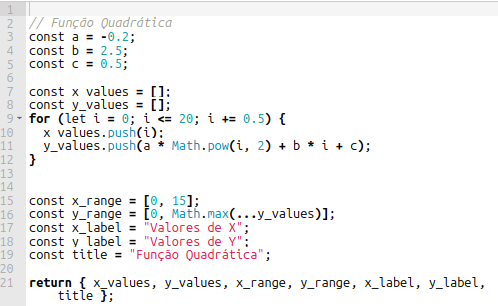
\includegraphics[keepaspectratio]{figs/padrao.png}}

}

\caption{\label{fig-padrao}Código padrão para a parábola, como exemplo
de uma estrutura de linguagem para \emph{JS}.}

\end{figure}%

\subsection*{Lógica de
programação}\label{luxf3gica-de-programauxe7uxe3o}
\addcontentsline{toc}{subsection}{Lógica de programação}

~~Vamos analisar o código da parábola por 3 \emph{``jeitos''}
crescentes.

\subsubsection*{1a. Visão do código}\label{a.-visuxe3o-do-cuxf3digo}
\addcontentsline{toc}{subsubsection}{1a. Visão do código}

~~O código modela uma parábola (\emph{y = ax²+bx+c}) com coeficientes
fixados no início. Inicialmente produz uma lista \emph{x} e outra
\emph{y}, define os limites que vão aparecer no gráfico, coloca alguns
nomes e depois desenha o gráfico.

~~Essa é descrição do \emph{algoritmo em linguagem natural}, uma
primeira aproximação entre a ideia que se deseja e sua formalização.

\subsubsection*{2a. Visão do código}\label{a.-visuxe3o-do-cuxf3digo-1}
\addcontentsline{toc}{subsubsection}{2a. Visão do código}

~~Pesando na estrutura da linguagem de programação, o código funciona
mais ou menos assim:

\begin{enumerate}
\def\labelenumi{\arabic{enumi}.}
\tightlist
\item
  Define-se primeiro os parâmetros da parábola como \emph{const}antes
  (\emph{declaração de variáveis});
\item
  Cria-se duas listas vazias onde será introduzidos os dados
  (\emph{vetores} - \emph{x e y});
\item
  Cria-se os valores para \emph{x} com um \emph{laço repetitivo for}
  (\emph{estrutura de controle});
\item
  Calcula-se os valores de \emph{y} com base na equação
  (\emph{cálculos});
\item
  Define-se os limites de valores de \emph{x} e \emph{y} para o gráfico;
\item
  Coloca-se rótulos no gráfico, como título e os nomes dos eixos;
\item
  Entrega-se o gráfico com os ítens acima.
\end{enumerate}

~~Essa forma de observar como o objeto é criado numa linguagem de
programação está inserida num conceito denominado \emph{pensamento
computacional (PC)}. Veja que a lógica desse \emph{PC} envolve dividir o
problema em partes e solucionar cada parte individualmente no algoritmo
(\emph{dividir para conquistar!}).

\subsubsection*{3a. Visão do código}\label{a.-visuxe3o-do-cuxf3digo-2}
\addcontentsline{toc}{subsubsection}{3a. Visão do código}

~~Uma outra forma de se abordar o código se dá pelo que se denomina
\emph{lógica de programação} ou \emph{pseudocódigo} (\emph{pseudo
linguagem}). Ao invés de se textualizar o que o código faz, como acima,
ou de se oferecer toda a sintaxe de seus comandos, busca-se descrevê-lo
combinando-se um pouco de ambos, linguagem natural e estrutura de
programação. Para o exemplo da parábola, a pseudolinguagem poderia ser:

\hfill\break

\begin{Shaded}
\begin{Highlighting}[]
\NormalTok{INÍCIO}

\SpecialCharTok{/}\ErrorTok{/} \DecValTok{1}\ErrorTok{)}\NormalTok{ Definir parâmetros da função quadrática y }\OtherTok{=}\NormalTok{ a·x² }\SpecialCharTok{+}\NormalTok{ b·x }\SpecialCharTok{+}\NormalTok{ c}
\NormalTok{a ← }\SpecialCharTok{{-}}\DecValTok{0}\NormalTok{,}\DecValTok{2}
\NormalTok{b ←  }\DecValTok{2}\NormalTok{,}\DecValTok{5}
\NormalTok{c ←  }\DecValTok{0}\NormalTok{,}\DecValTok{5}

\SpecialCharTok{/}\ErrorTok{/} \DecValTok{2}\ErrorTok{)}\NormalTok{ Preparar vetores de dados}
\NormalTok{x\_values ← lista vazia}
\NormalTok{y\_values ← lista vazia}

\SpecialCharTok{/}\ErrorTok{/} \DecValTok{3}\ErrorTok{)}\NormalTok{ Varredura do domínio}\SpecialCharTok{:}\NormalTok{ gerar pontos de x de }\DecValTok{0}\NormalTok{ até }\DecValTok{20}\NormalTok{, passo }\DecValTok{0}\NormalTok{,}\DecValTok{5}
\NormalTok{PARA x DE }\DecValTok{0}\NormalTok{ ATÉ }\DecValTok{20}\NormalTok{ PASSO }\DecValTok{0}\NormalTok{,}\DecValTok{5}\NormalTok{ FAÇA}
    \SpecialCharTok{/}\ErrorTok{/} \FloatTok{3.1}\ErrorTok{)}\NormalTok{ Registrar o x}
\NormalTok{    anexar x EM x\_values}

    \SpecialCharTok{/}\ErrorTok{/} \FloatTok{3.2}\ErrorTok{)}\NormalTok{ Calcular }\FunctionTok{y}\NormalTok{(x) }\OtherTok{=}\NormalTok{ a·x² }\SpecialCharTok{+}\NormalTok{ b·x }\SpecialCharTok{+}\NormalTok{ c}
\NormalTok{    y ← a }\SpecialCharTok{*}\NormalTok{ (x}\SpecialCharTok{\^{}}\DecValTok{2}\NormalTok{) }\SpecialCharTok{+}\NormalTok{ b }\SpecialCharTok{*}\NormalTok{ x }\SpecialCharTok{+}\NormalTok{ c}

    \SpecialCharTok{/}\ErrorTok{/} \FloatTok{3.3}\ErrorTok{)}\NormalTok{ Registrar o y}
\NormalTok{    anexar y EM y\_values}
\NormalTok{FIM}\SpecialCharTok{{-}}\NormalTok{PARA}

\SpecialCharTok{/}\ErrorTok{/} \DecValTok{4}\ErrorTok{)}\NormalTok{ Definir faixas de }\FunctionTok{eixos}\NormalTok{ (range) e rótulos}
\NormalTok{x\_range ← [}\DecValTok{0}\NormalTok{, }\DecValTok{15}\NormalTok{]               }\SpecialCharTok{/}\ErrorTok{/}\NormalTok{ mostrar no gráfico apenas x entre }\DecValTok{0}\NormalTok{ e }\DecValTok{15}
\NormalTok{y\_range ← [}\DecValTok{0}\NormalTok{, MÁXIMO(y\_values)] }\SpecialCharTok{/}\ErrorTok{/}\NormalTok{ mínimo fixo em }\DecValTok{0}\NormalTok{; máximo conforme dados}

\NormalTok{x\_label ← }\StringTok{"Valores de X"}
\NormalTok{y\_label ← }\StringTok{"Valores de Y"}
\NormalTok{title   ← }\StringTok{"Função Quadrática"}

\SpecialCharTok{/}\ErrorTok{/} \DecValTok{5}\ErrorTok{)}\NormalTok{ Entregar o }\StringTok{"pacote de saída"}\NormalTok{ para o mecanismo gráfico}
\NormalTok{RETORNAR \{}
\NormalTok{  x\_values, y\_values,}
\NormalTok{  x\_range, y\_range,}
\NormalTok{  x\_label, y\_label,}
\NormalTok{  title}
\NormalTok{\}}

\NormalTok{FIM}
\end{Highlighting}
\end{Shaded}

\hfill\break

~~Perceba então a \emph{``escadinha''} de linguagem que se forma entre a
ideia original e o algoritmo final:

~~Natural → Pseudocódigo → Código real

\bookmarksetup{startatroot}

\chapter{Um pouco de estrutura
JavaScript}\label{um-pouco-de-estrutura-javascript}

\section{Separação de comandos e inserção de
comentários}\label{separauxe7uxe3o-de-comandos-e-inseruxe7uxe3o-de-comentuxe1rios}

~~Os comandos em \emph{JS} são separados por \emph{ponto e vírgula,
``;''}.

~~Já os comentários constituem trechos não interpretados, comumente
utilizados em programação. Comentários são tremendamente úteis quando se
deseja colocar um título no \emph{script} de código, por exemplo, para
explicar determinada ação, apontar uma futura melhoria, entre muitos. Em
\emph{JS} são alternativamente inseridos por \emph{'' // ``} antes de
cada comando, ou por \emph{'' /}\ldots.\emph{/ ``}, para comentários
mais extensos.

\section{Declaração de
variáveis}\label{declarauxe7uxe3o-de-variuxe1veis}

~~Entre os diversos tipos de variáveis em \emph{JS}, duas são
frequentemente utilizadas: \emph{const} e \emph{let}. A variável
\emph{const} é utilizada para se atribuir um valor fixo a uma variável
no código, enquanto a variável \emph{let} é empregada quando se deseja
reatribuir um valor a ela, por meio de algum cálculo ou laço iterativo.
Exemplificando, quando se deseja variáveis de controle que mudam ao
longo do tempo (sliders, passos, intervalos).

\subsection{``Botando a mão na massa''}\label{botando-a-muxe3o-na-massa}

Como esse treinamento envolve instruir o algoritmo com uma
\emph{entrada} para que sua interpretação resulte numa \emph{saída},
aqui propomos essa última pelo comando \texttt{print}, como segue.

\begin{Shaded}
\begin{Highlighting}[]
\KeywordTok{const}\NormalTok{ a }\OperatorTok{=} \OperatorTok{{-}}\FloatTok{0.2}\OperatorTok{;}
\FunctionTok{print}\NormalTok{(a)}
\end{Highlighting}
\end{Shaded}

~~Para esse treinamento utilizaremos o \emph{JSPlotly} personalizado
abaixo. Assim, teste a atribuição da variável \emph{const} e do comando
\texttt{print} por cópia do trecho acima e cola no campo de texto
\emph{ÁREA PARA DIGITAR COMANDOS} do script que segue, seguido de
\emph{add}:

\hfill\break

~~Existem outros comandos de saída para \emph{JS}, como
\texttt{console.log()} e \texttt{document.body.appendChild()}, mas não
utilizáveis pelo aplicativo.

~~Pode-se atribuir também um texto para apresentar a constante, veja:

\hfill\break

\begin{Shaded}
\begin{Highlighting}[]
\KeywordTok{const}\NormalTok{ a }\OperatorTok{=} \OperatorTok{{-}}\FloatTok{0.2}\OperatorTok{;}
\FunctionTok{print}\NormalTok{(}\StringTok{"constante:"}\OperatorTok{,}\NormalTok{a)}
\end{Highlighting}
\end{Shaded}

~~E também realizar cálculos diretos, veja:

\hfill\break

\begin{Shaded}
\begin{Highlighting}[]
\KeywordTok{const}\NormalTok{ a }\OperatorTok{=} \DecValTok{5}\OperatorTok{;} \CommentTok{// variável constante (não se altera ao longo do código)}
\KeywordTok{const}\NormalTok{ b }\OperatorTok{=} \DecValTok{10}\OperatorTok{;} \CommentTok{// variável que pode alterar seu valor no código}
\FunctionTok{print}\NormalTok{(a}\OperatorTok{*}\NormalTok{b)}
\end{Highlighting}
\end{Shaded}

~~Outro exemplo, com inserção de texto antes do resultado:

\begin{Shaded}
\begin{Highlighting}[]
\KeywordTok{let}\NormalTok{ a }\OperatorTok{=} \DecValTok{5}\OperatorTok{;}
\KeywordTok{const}\NormalTok{ b }\OperatorTok{=} \DecValTok{10}\OperatorTok{;}

\KeywordTok{let}\NormalTok{ resultado }\OperatorTok{=}\NormalTok{ a }\OperatorTok{+}\NormalTok{ b}\OperatorTok{;}
\FunctionTok{print}\NormalTok{(}\StringTok{"Soma de a + b:"}\OperatorTok{,}\NormalTok{ resultado)}\OperatorTok{;}
\end{Highlighting}
\end{Shaded}

\hfill\break

\subsection{\texorpdfstring{\emph{const} X
\emph{let}}{const X let}}\label{const-x-let}

~~Pode parecer que \emph{const} e \emph{let} são distintas apenas na
aparência, já que operam de modo intercambiável. Contudo, para
explicitar a diferença entre os dois comandos, apague o ecrã gráfico
(\emph{clean}) e substitua a linha de código da seção anterior pela que
segue na \emph{ÁREA PARA DIGITAR COMANDOS} do script:

\begin{Shaded}
\begin{Highlighting}[]
\KeywordTok{let}\NormalTok{ passo }\OperatorTok{=} \FloatTok{0.5}\OperatorTok{;}          \CommentTok{// usuário pode alterar}
\KeywordTok{let}\NormalTok{ x0 }\OperatorTok{=} \DecValTok{0}\OperatorTok{;}      \CommentTok{// domínios dinâmicos}
\FunctionTok{print}\NormalTok{(passo}\OperatorTok{,}\NormalTok{ x0) }

\CommentTok{// ... mais tarde:}
\NormalTok{passo }\OperatorTok{=} \FloatTok{0.2}\OperatorTok{;}\NormalTok{ x0 }\OperatorTok{=} \DecValTok{30}\OperatorTok{;}
\FunctionTok{print}\NormalTok{(passo}\OperatorTok{,}\NormalTok{ x0)}
\end{Highlighting}
\end{Shaded}

~~~~Aparentemente, o resultado sugere que na prática nada muda, sendo a
diferença mais centrada na clareza e segurança do código. Mas não é bem
assim. Experimente agora trocar o campo pra executar o código abaixo:

\begin{Shaded}
\begin{Highlighting}[]
\KeywordTok{let}\NormalTok{ contador }\OperatorTok{=} \DecValTok{0}\OperatorTok{;}
\NormalTok{contador }\OperatorTok{+=} \DecValTok{1}\OperatorTok{;}
\FunctionTok{print}\NormalTok{(}\StringTok{"Contador:"}\OperatorTok{,}\NormalTok{ contador)}\OperatorTok{;}
\end{Highlighting}
\end{Shaded}

~~Agora substitua a variável do \emph{``contador''} para \emph{const} ao
invés de \emph{let}. O resultado incorrerá no erro abaixo:

\hfill\break

\begin{figure}

\centering{

\pandocbounded{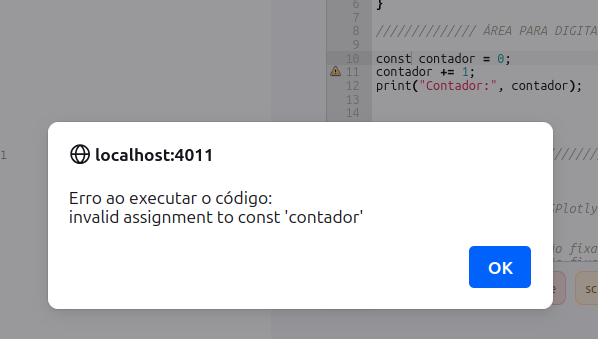
\includegraphics[keepaspectratio]{figs/erroConst.png}}

}

\caption{\label{fig-erroConst}Erro gerado quando se substitui a variável
\emph{let} por \emph{const} num trecho de reatribuição de valor.}

\end{figure}%

~~Resumindo: para constantes, use \emph{const} e para variável
reatribuível use \emph{let}.

\section{Tipos de dados}\label{tipos-de-dados}

~~Como é comum para outras linguagens, \emph{JavaScript} possui alguns
tipos comuns para definição de dados. Para uso de \texttt{Plotly.js},
são bem significativos:

\begin{Shaded}
\begin{Highlighting}[]
\NormalTok{Number }\CommentTok{\# número}
\NormalTok{String }\CommentTok{\# texto: representado entre aspas ( " " )}
\NormalTok{Boolean }\CommentTok{\# true/false ("branching")}
\NormalTok{Object  }\CommentTok{\# internos (built{-}in) ou externos (user{-}defined)}
\NormalTok{Built}\SpecialCharTok{{-}}\ControlFlowTok{in} \CommentTok{\# objects, arrays, dates, maps, etc}
\end{Highlighting}
\end{Shaded}

~~Seguem alguns exemplos práticos. Experimente trocar cada um na saída
\texttt{print}:

\begin{Shaded}
\begin{Highlighting}[]
\CommentTok{// Numbers:}
\KeywordTok{let}\NormalTok{ comprimento }\OperatorTok{=} \DecValTok{116}\OperatorTok{;}
\KeywordTok{let}\NormalTok{ peso }\OperatorTok{=} \DecValTok{75}\OperatorTok{;}

\CommentTok{// Strings:}
\KeywordTok{let}\NormalTok{ color }\OperatorTok{=} \StringTok{"Yellow"}\OperatorTok{;}
\KeywordTok{let}\NormalTok{ lastName }\OperatorTok{=} \StringTok{"Johnson"}\OperatorTok{;}

\CommentTok{// Booleans}
\KeywordTok{let}\NormalTok{ x }\OperatorTok{=} \KeywordTok{true}\OperatorTok{;}
\KeywordTok{let}\NormalTok{ y }\OperatorTok{=} \KeywordTok{false}\OperatorTok{;}

\CommentTok{// Object:}
\KeywordTok{const}\NormalTok{ membro }\OperatorTok{=}\NormalTok{ \{}\DataTypeTok{firstName}\OperatorTok{:}\StringTok{"John"}\OperatorTok{,} \DataTypeTok{lastName}\OperatorTok{:}\StringTok{"Doe"}\NormalTok{\}}\OperatorTok{;}

\CommentTok{// Array object:}
\KeywordTok{const}\NormalTok{ carros }\OperatorTok{=}\NormalTok{ [}\StringTok{"Saab"}\OperatorTok{,} \StringTok{"Volvo"}\OperatorTok{,} \StringTok{"BMW"}\NormalTok{]}\OperatorTok{;}

\CommentTok{// Date object:}
    \KeywordTok{const}\NormalTok{ datas }\OperatorTok{=} \KeywordTok{new} \BuiltInTok{Date}\NormalTok{(}\StringTok{"2022{-}03{-}25"}\NormalTok{)}\OperatorTok{;}

\CommentTok{// Saídas:}
\FunctionTok{print}\NormalTok{(comprimento)}
\end{Highlighting}
\end{Shaded}

\section{Constantes}\label{constantes}

~~Por vezes é necessária a inserção de constantes matemáticas em
equações para plotagem ou cálculos. Seguem alguns exemplos. Para a saída
no \emph{JSPlotly} customizado abaixo, basta o bom e velho
\texttt{print} que segue ao também bom e velho \emph{clean}.

\begin{Shaded}
\begin{Highlighting}[]
\BuiltInTok{Math}\OperatorTok{.}\ConstantTok{PI} \OperatorTok{{-}}\NormalTok{ valor }\FunctionTok{de}\NormalTok{ (pi)}\OperatorTok{,}\NormalTok{ aproximadamente }\FloatTok{3.14159}
\BuiltInTok{Math}\OperatorTok{.}\ConstantTok{E} \OperatorTok{{-}}\NormalTok{ valor da constante de Euler}\OperatorTok{,}\NormalTok{ aproximadamente }\FloatTok{2.71828}
\BuiltInTok{Math}\OperatorTok{.}\ConstantTok{LN2} \OperatorTok{{-}}\NormalTok{ logaritmo natural de }\DecValTok{2}\OperatorTok{,}\NormalTok{ aproximadamente }\FloatTok{0.693}
\BuiltInTok{Math}\OperatorTok{.}\ConstantTok{LN10} \OperatorTok{{-}}\NormalTok{ logaritmo natural de }\DecValTok{10}\OperatorTok{,}\NormalTok{ aproximadamente }\FloatTok{2.302}
\BuiltInTok{Math}\OperatorTok{.}\ConstantTok{LOG2E} \OperatorTok{{-}}\NormalTok{ logaritmo de e na base }\DecValTok{2}\OperatorTok{,}\NormalTok{ aproximadamente }\FloatTok{1.442}
\BuiltInTok{Math}\OperatorTok{.}\ConstantTok{LOG10E} \OperatorTok{{-}}\NormalTok{ logaritmo de e na base }\DecValTok{10}\OperatorTok{,}\NormalTok{ aproximadamente }\FloatTok{0.434}
\BuiltInTok{Number}\OperatorTok{.}\ConstantTok{MAX\_VALUE} \OperatorTok{{-}}\NormalTok{ maior número positivo}
\BuiltInTok{Number}\OperatorTok{.}\ConstantTok{MIN\_VALUE} \OperatorTok{{-}}\NormalTok{ menor número positivo}\OperatorTok{...}
\end{Highlighting}
\end{Shaded}

~~Para constantes naturais, contudo, é necessário defini-las
antecipadamente, como em:

\begin{Shaded}
\begin{Highlighting}[]
\CommentTok{// Definindo constantes físico{-}químicas comuns}
\KeywordTok{const}\NormalTok{ Avogadro }\OperatorTok{=} \FloatTok{6.02214076e23}\OperatorTok{;}  \CommentTok{// Número de Avogadro (mol⁻¹)}
\KeywordTok{const}\NormalTok{ Boltzmann }\OperatorTok{=} \FloatTok{1.380649e{-}23}\OperatorTok{;}  \CommentTok{// Constante de Boltzmann (J/K)}
\KeywordTok{const}\NormalTok{ Planck }\OperatorTok{=} \FloatTok{6.62607015e{-}34}\OperatorTok{;}   \CommentTok{// Constante de Planck (J·s)}
\KeywordTok{const}\NormalTok{ gas }\OperatorTok{=} \FloatTok{8.31446}\OperatorTok{;}    \CommentTok{// Constante dos gases ideais (J/(mol·K))}
\KeywordTok{const}\NormalTok{ luz }\OperatorTok{=} \DecValTok{299792458}\OperatorTok{;} \CommentTok{// Velocidade da luz no vácuo (m/s)}
\end{Highlighting}
\end{Shaded}

\bookmarksetup{startatroot}

\chapter{Mais estrutura}\label{mais-estrutura}

~~Neste capítulo será ilustrado a estrutura de \emph{JavaScript} para
aritmética, \emph{arrays} (vetores), funções, geração de números
aleatórios, e objetos.

~~Como são exemplificados diversas linhas para cada, e partindo-se do
pressuposto que você já deve estar um pouco cansado de utilizar o
\texttt{print} recursivamente (embora tivesse sido intencional, he, he),
segue um trecho que permite um copia/colar direto para todos os comandos
de uma só vez.

~~Na prática, é só separar cada comando por \emph{``;'} seguido de
\texttt{print()}.

\hfill\break

\section{Aritmética}\label{aritmuxe9tica}

~~Diversas operações matemáticas são possíveis, quer pelo
\emph{JavaScript} puro, quer pela instalação de bibliotecas específicas,
tais como \emph{mathjs} ou \emph{numjs}. Seguem algumas operações
básicas, para testar no \emph{JSPlotly} customizado, também abaixo:

\begin{Shaded}
\begin{Highlighting}[]
\KeywordTok{let}\NormalTok{ resultado }\OperatorTok{=} \DecValTok{0}\OperatorTok{;}

\NormalTok{resultado }\OperatorTok{=} \DecValTok{5} \OperatorTok{+} \DecValTok{3}\OperatorTok{;}                 \FunctionTok{print}\NormalTok{(}\StringTok{"5 + 3 = "}\OperatorTok{,}\NormalTok{ resultado)}\OperatorTok{;}          \CommentTok{// 8}
\NormalTok{resultado }\OperatorTok{=} \DecValTok{10} \OperatorTok{{-}} \DecValTok{4}\OperatorTok{;}                \FunctionTok{print}\NormalTok{(}\StringTok{"10 {-} 4 = "}\OperatorTok{,}\NormalTok{ resultado)}\OperatorTok{;}          \CommentTok{// 6}
\NormalTok{resultado }\OperatorTok{=} \DecValTok{6} \OperatorTok{*} \DecValTok{7}\OperatorTok{;}                 \FunctionTok{print}\NormalTok{(}\StringTok{"6 * 7 = "}\OperatorTok{,}\NormalTok{ resultado)}\OperatorTok{;}           \CommentTok{// 42}
\NormalTok{resultado }\OperatorTok{=} \DecValTok{20} \OperatorTok{/} \DecValTok{5}\OperatorTok{;}                \FunctionTok{print}\NormalTok{(}\StringTok{"20 / 5 = "}\OperatorTok{,}\NormalTok{ resultado)}\OperatorTok{;}          \CommentTok{// 4}
\NormalTok{resultado }\OperatorTok{=} \DecValTok{17} \OperatorTok{\%} \DecValTok{3}\OperatorTok{;}                \FunctionTok{print}\NormalTok{(}\StringTok{"17 \% 3 = "}\OperatorTok{,}\NormalTok{ resultado)}\OperatorTok{;}          \CommentTok{// 2}
\NormalTok{resultado }\OperatorTok{=} \DecValTok{2} \OperatorTok{**} \DecValTok{3}\OperatorTok{;}                \FunctionTok{print}\NormalTok{(}\StringTok{"2 ** 3 = "}\OperatorTok{,}\NormalTok{ resultado)}\OperatorTok{;}          \CommentTok{// 8}
\KeywordTok{let}\NormalTok{ contador }\OperatorTok{=} \DecValTok{5}\OperatorTok{;}\NormalTok{ contador}\OperatorTok{++;}      \FunctionTok{print}\NormalTok{(}\StringTok{"contador++ = "}\OperatorTok{,}\NormalTok{ contador)}\OperatorTok{;}       \CommentTok{// 6}
\KeywordTok{let}\NormalTok{ decrementar }\OperatorTok{=} \DecValTok{8}\OperatorTok{;}\NormalTok{ decrementar}\OperatorTok{{-}{-};}\FunctionTok{print}\NormalTok{(}\StringTok{"decrementar{-}{-} = "}\OperatorTok{,}\NormalTok{ decrementar)}\OperatorTok{;} \CommentTok{// 7}
\KeywordTok{let}\NormalTok{ soma }\OperatorTok{=} \DecValTok{10}\OperatorTok{;}\NormalTok{ soma }\OperatorTok{+=} \DecValTok{5}\OperatorTok{;}          \FunctionTok{print}\NormalTok{(}\StringTok{"soma += 5 = "}\OperatorTok{,}\NormalTok{ soma)}\OperatorTok{;}            \CommentTok{// 15}
\KeywordTok{let}\NormalTok{ diferenca }\OperatorTok{=} \DecValTok{20}\OperatorTok{;}\NormalTok{ diferenca }\OperatorTok{{-}=} \DecValTok{7}\OperatorTok{;}\FunctionTok{print}\NormalTok{(}\StringTok{"diferença {-}= 7 = "}\OperatorTok{,}\NormalTok{ diferenca)}\OperatorTok{;}   \CommentTok{// 13}
\KeywordTok{let}\NormalTok{ produto }\OperatorTok{=} \DecValTok{3}\OperatorTok{;}\NormalTok{ produto }\OperatorTok{*=} \DecValTok{4}\OperatorTok{;}     \FunctionTok{print}\NormalTok{(}\StringTok{"produto *= 4 = "}\OperatorTok{,}\NormalTok{ produto)}\OperatorTok{;}       \CommentTok{// 12}
\KeywordTok{let}\NormalTok{ quociente }\OperatorTok{=} \DecValTok{24}\OperatorTok{;}\NormalTok{ quociente }\OperatorTok{/=} \DecValTok{3}\OperatorTok{;}\FunctionTok{print}\NormalTok{(}\StringTok{"quociente /= 3 = "}\OperatorTok{,}\NormalTok{ quociente)}\OperatorTok{;}   \CommentTok{// 8}
\NormalTok{resultado }\OperatorTok{=} \BuiltInTok{Math}\OperatorTok{.}\FunctionTok{sqrt}\NormalTok{(}\DecValTok{25}\NormalTok{)}\OperatorTok{;}         \FunctionTok{print}\NormalTok{(}\StringTok{"sqrt(25) = "}\OperatorTok{,}\NormalTok{ resultado)}\OperatorTok{;}         \CommentTok{// 5}
\NormalTok{resultado }\OperatorTok{=} \BuiltInTok{Math}\OperatorTok{.}\FunctionTok{abs}\NormalTok{(}\OperatorTok{{-}}\DecValTok{15}\NormalTok{)}\OperatorTok{;}         \FunctionTok{print}\NormalTok{(}\StringTok{"abs({-}15) = "}\OperatorTok{,}\NormalTok{ resultado)}\OperatorTok{;}         \CommentTok{// 15}
\NormalTok{resultado }\OperatorTok{=} \BuiltInTok{Math}\OperatorTok{.}\FunctionTok{floor}\NormalTok{(}\FloatTok{7.8}\NormalTok{)}\OperatorTok{;}       \FunctionTok{print}\NormalTok{(}\StringTok{"floor(7.8) = "}\OperatorTok{,}\NormalTok{ resultado)}\OperatorTok{;}       \CommentTok{// 7}
\NormalTok{resultado }\OperatorTok{=} \BuiltInTok{Math}\OperatorTok{.}\FunctionTok{ceil}\NormalTok{(}\FloatTok{7.2}\NormalTok{)}\OperatorTok{;}        \FunctionTok{print}\NormalTok{(}\StringTok{"ceil(7.2) = "}\OperatorTok{,}\NormalTok{ resultado)}\OperatorTok{;}        \CommentTok{// 8}
\NormalTok{resultado }\OperatorTok{=} \BuiltInTok{Math}\OperatorTok{.}\FunctionTok{round}\NormalTok{(}\FloatTok{9.4}\NormalTok{)}\OperatorTok{;}       \FunctionTok{print}\NormalTok{(}\StringTok{"round(9.4) = "}\OperatorTok{,}\NormalTok{ resultado)}\OperatorTok{;}       \CommentTok{// 9}
\NormalTok{resultado }\OperatorTok{=} \BuiltInTok{Math}\OperatorTok{.}\FunctionTok{max}\NormalTok{(}\DecValTok{42}\OperatorTok{,} \DecValTok{27}\NormalTok{)}\OperatorTok{;}      \FunctionTok{print}\NormalTok{(}\StringTok{"max(42,27) = "}\OperatorTok{,}\NormalTok{ resultado)}\OperatorTok{;}       \CommentTok{// 42}
\NormalTok{resultado }\OperatorTok{=} \BuiltInTok{Math}\OperatorTok{.}\FunctionTok{min}\NormalTok{(}\DecValTok{42}\OperatorTok{,} \DecValTok{27}\NormalTok{)}\OperatorTok{;}      \FunctionTok{print}\NormalTok{(}\StringTok{"min(42,27) = "}\OperatorTok{,}\NormalTok{ resultado)}\OperatorTok{;}       \CommentTok{// 27}
\NormalTok{resultado }\OperatorTok{=} \BuiltInTok{Math}\OperatorTok{.}\FunctionTok{sin}\NormalTok{(}\BuiltInTok{Math}\OperatorTok{.}\ConstantTok{PI}\OperatorTok{/}\DecValTok{2}\NormalTok{)}\OperatorTok{;}   \FunctionTok{print}\NormalTok{(}\StringTok{"sin(π/2) = "}\OperatorTok{,}\NormalTok{ resultado)}\OperatorTok{;} 
\end{Highlighting}
\end{Shaded}

\section{Arrays}\label{arrays}

~~Um \emph{array} em \emph{JavaScript} representa uma estrutura de dados
para armazenamento de elementos ordenados. Esses elementos podem
envolver qualquer tipo de dado, como números, strings, objetos, etc. Na
prática, um \emph{array} pode ser criado, acessado, filtrado, ou
mapeado. Seguem exemplos:

\subsubsection*{Criação}\label{criauxe7uxe3o}
\addcontentsline{toc}{subsubsection}{Criação}

\begin{Shaded}
\begin{Highlighting}[]
\KeywordTok{const}\NormalTok{ numeros }\OperatorTok{=}\NormalTok{ [}\DecValTok{1}\OperatorTok{,} \DecValTok{2}\OperatorTok{,} \DecValTok{3}\OperatorTok{,} \DecValTok{4}\OperatorTok{,} \DecValTok{5}\NormalTok{]}\OperatorTok{;}
\KeywordTok{const}\NormalTok{ cores }\OperatorTok{=}\NormalTok{ [}\StringTok{\textquotesingle{}vermelho\textquotesingle{}}\OperatorTok{,} \StringTok{\textquotesingle{}verde\textquotesingle{}}\OperatorTok{,} \StringTok{\textquotesingle{}azul\textquotesingle{}}\NormalTok{]}\OperatorTok{;}
\end{Highlighting}
\end{Shaded}

\subsubsection*{Acesso}\label{acesso}
\addcontentsline{toc}{subsubsection}{Acesso}

\begin{Shaded}
\begin{Highlighting}[]
\FunctionTok{print}\NormalTok{(numeros[}\DecValTok{0}\NormalTok{])}\OperatorTok{;}
\FunctionTok{print}\NormalTok{(cores[}\DecValTok{2}\NormalTok{])}\OperatorTok{;}
\end{Highlighting}
\end{Shaded}

\subsubsection*{\texorpdfstring{Mapeamento
(\texttt{map})}{Mapeamento (map)}}\label{mapeamento-map}
\addcontentsline{toc}{subsubsection}{Mapeamento (\texttt{map})}

\begin{Shaded}
\begin{Highlighting}[]
\KeywordTok{const}\NormalTok{ numeros }\OperatorTok{=}\NormalTok{ [}\DecValTok{1}\OperatorTok{,} \DecValTok{2}\OperatorTok{,} \DecValTok{3}\OperatorTok{,} \DecValTok{4}\OperatorTok{,} \DecValTok{5}\NormalTok{]}\OperatorTok{;}
\KeywordTok{const}\NormalTok{ quadrados }\OperatorTok{=}\NormalTok{ numeros}\OperatorTok{.}\FunctionTok{map}\NormalTok{(numero }\KeywordTok{=\textgreater{}}\NormalTok{ numero }\OperatorTok{*}\NormalTok{ numero)}\OperatorTok{;}
\FunctionTok{print}\NormalTok{(quadrados)}\OperatorTok{;}
\end{Highlighting}
\end{Shaded}

\subsection{Uma palavrinha sobre
métodos}\label{uma-palavrinha-sobre-muxe9todos}

~~Observe que, diferente do que já foi explicitado, agora aparece um
comando múltiplo, como \emph{``numeros.map''}. Existe uma infinidade de
comandos com esta sintaxe em \emph{JS}. Ele representa a função que será
aplicada a cada elemento do array \emph{numeros} pelo \emph{método map}.
Além disso, surge a sintaxe \emph{``=\textgreater{}''} ou sintaxe de
\emph{arrow function} (função de seta), uma forma concisa de atribuir um
mapeamento. Assim, o comando inteiro:

\begin{Shaded}
\begin{Highlighting}[]
\NormalTok{const quadrados = numeros.map(numero =\textgreater{} numero * numero)}

\NormalTok{...traduz{-}se como...}

\NormalTok{"recebe um numero como parâmetro e retorna o seu quadrado (numero * numero)"}
\end{Highlighting}
\end{Shaded}

~~Esmiuçando um pouquinho mais, o \emph{método map()} é chamado no
\emph{array numeros} (um \emph{Array.prototype}). Ele itera sobre cada
elemento do array original, aplica uma função a cada um deles e retorna
um novo array com os resultados. Assim, \emph{numero =\textgreater{}
numero } numero* é a \emph{função de seta}. E nesse caso, \emph{numero}
é o parâmetro de entrada da função, um atalho para o elemento atual do
\emph{array} sendo processado pelo \emph{map}. Em adição,
\emph{``=\textgreater{}''} representa o separador entre o(s)
parâmetro(s) e o corpo da função. Finalmente, \emph{``numero * numero''}
é a expressão que é executada, com o resultado sendo retornado pela
função.

\hfill\break

~~Seguem outros exemplos para arrays e mapeamento:

\hfill\break

\begin{Shaded}
\begin{Highlighting}[]
 \KeywordTok{const}\NormalTok{ x }\OperatorTok{=}\NormalTok{ [}\DecValTok{0}\OperatorTok{,} \DecValTok{1}\OperatorTok{,} \DecValTok{2}\OperatorTok{,} \DecValTok{3}\OperatorTok{,} \DecValTok{4}\NormalTok{]}\OperatorTok{;}
 \KeywordTok{const}\NormalTok{ y }\OperatorTok{=}\NormalTok{ x}\OperatorTok{.}\FunctionTok{map}\NormalTok{(valor }\KeywordTok{=\textgreater{}} \BuiltInTok{Math}\OperatorTok{.}\FunctionTok{pow}\NormalTok{(}\DecValTok{2}\OperatorTok{,}\NormalTok{ valor))}
 \FunctionTok{print}\NormalTok{(y)}\OperatorTok{;}
\end{Highlighting}
\end{Shaded}

\begin{Shaded}
\begin{Highlighting}[]
\KeywordTok{const}\NormalTok{ Vmax }\OperatorTok{=} \DecValTok{100}\OperatorTok{;}
\KeywordTok{const}\NormalTok{ Km }\OperatorTok{=} \DecValTok{10}\OperatorTok{;}
\KeywordTok{const}\NormalTok{ S\_values }\OperatorTok{=} \BuiltInTok{Array}\OperatorTok{.}\FunctionTok{from}\NormalTok{(\{}\DataTypeTok{length}\OperatorTok{:} \DecValTok{10}\NormalTok{\}}\OperatorTok{,}\NormalTok{ (\_}\OperatorTok{,}\NormalTok{ i) }\KeywordTok{=\textgreater{}}\NormalTok{ i }\OperatorTok{*} \DecValTok{5}\NormalTok{)}\OperatorTok{;}

\KeywordTok{const}\NormalTok{ V\_values }\OperatorTok{=}\NormalTok{ S\_values}\OperatorTok{.}\FunctionTok{map}\NormalTok{(S }\KeywordTok{=\textgreater{}}\NormalTok{ (Vmax }\OperatorTok{*}\NormalTok{ S) }\OperatorTok{/}\NormalTok{ (Km }\OperatorTok{+}\NormalTok{ S))}\OperatorTok{;}

\FunctionTok{print}\NormalTok{(}\StringTok{"Valores de S:"}\OperatorTok{,}\NormalTok{ S\_values)}\OperatorTok{;}
\FunctionTok{print}\NormalTok{(}\StringTok{"Valores de V:"}\OperatorTok{,}\NormalTok{ V\_values)}\OperatorTok{;}
\end{Highlighting}
\end{Shaded}

\hfill\break

\subsubsection*{Filtragem}\label{filtragem}
\addcontentsline{toc}{subsubsection}{Filtragem}

\begin{Shaded}
\begin{Highlighting}[]
\KeywordTok{const}\NormalTok{ numeros }\OperatorTok{=}\NormalTok{ [}\DecValTok{1}\OperatorTok{,} \DecValTok{2}\OperatorTok{,} \DecValTok{3}\OperatorTok{,} \DecValTok{4}\OperatorTok{,} \DecValTok{5}\NormalTok{]}\OperatorTok{;}
\KeywordTok{const}\NormalTok{ pares }\OperatorTok{=}\NormalTok{ numeros}\OperatorTok{.}\FunctionTok{filter}\NormalTok{(numero }\KeywordTok{=\textgreater{}}\NormalTok{ numero }\OperatorTok{\%} \DecValTok{2} \OperatorTok{===} \DecValTok{0}\NormalTok{)}\OperatorTok{;}  \CommentTok{// (\textasciigrave{}filter\textasciigrave{})}
\FunctionTok{print}\NormalTok{(pares)}\OperatorTok{;}

\NormalTok{numeros}\OperatorTok{.}\FunctionTok{forEach}\NormalTok{(numero }\KeywordTok{=\textgreater{}} \FunctionTok{print}\NormalTok{(numero }\OperatorTok{*} \DecValTok{2}\NormalTok{))}\OperatorTok{;}  \CommentTok{// \textasciigrave{}forEach()\textasciigrave{}}
\end{Highlighting}
\end{Shaded}

\hfill\break

\subsection{Um pouco mais sobre sobre os métodos ilustrados
acima}\label{um-pouco-mais-sobre-sobre-os-muxe9todos-ilustrados-acima}

~~Com o mesmo raciocínio empregado, os métodos empregados acima podem
ser traduzidos como:

\hfill\break

\begin{Shaded}
\begin{Highlighting}[]
\FloatTok{1.}  \KeywordTok{const}\NormalTok{ y }\OperatorTok{=}\NormalTok{ x}\OperatorTok{.}\FunctionTok{map}\NormalTok{(valor }\KeywordTok{=\textgreater{}} \BuiltInTok{Math}\OperatorTok{.}\FunctionTok{pow}\NormalTok{(}\DecValTok{2}\OperatorTok{,}\NormalTok{ valor))}
\OperatorTok{...}
\NormalTok{Cria um novo array y aplicando }\BuiltInTok{Array}\OperatorTok{.}\AttributeTok{prototype}\OperatorTok{.}\AttributeTok{map}\NormalTok{ sobre x}\OperatorTok{:}\NormalTok{ para cada valor}\OperatorTok{,}\NormalTok{ usa }\BuiltInTok{Math}\OperatorTok{.}\FunctionTok{pow}\NormalTok{(base}\OperatorTok{,}\NormalTok{ expoente) para calcular }\DecValTok{2}\OperatorTok{\^{}}\NormalTok{valor}\OperatorTok{;}

\FloatTok{2.} \KeywordTok{const}\NormalTok{ S\_values }\OperatorTok{=} \BuiltInTok{Array}\OperatorTok{.}\FunctionTok{from}\NormalTok{(\{}\DataTypeTok{length}\OperatorTok{:} \DecValTok{10}\NormalTok{\}}\OperatorTok{,}\NormalTok{ (\_}\OperatorTok{,}\NormalTok{ i) }\KeywordTok{=\textgreater{}}\NormalTok{ i }\OperatorTok{*} \DecValTok{5}\NormalTok{)}\OperatorTok{;}
\OperatorTok{...}
\NormalTok{Usa }\BuiltInTok{Array}\OperatorTok{.}\AttributeTok{from}\NormalTok{ com o objeto \{ }\DataTypeTok{length}\OperatorTok{:} \DecValTok{10}\NormalTok{ \} (propriedade length) e uma função }\FunctionTok{mapeadora}\NormalTok{ (\_}\OperatorTok{,}\NormalTok{ i) para gerar }\DecValTok{10}\NormalTok{ valores}\OperatorTok{,}\NormalTok{ cada um igual a índice multiplicado por }\DecValTok{5}\NormalTok{ (× }\DecValTok{5}\NormalTok{) → [}\DecValTok{0}\OperatorTok{,}\DecValTok{5}\OperatorTok{,}\DecValTok{10}\OperatorTok{,...,}\DecValTok{45}\NormalTok{]}\OperatorTok{;}

\FloatTok{3.} \KeywordTok{const}\NormalTok{ pares }\OperatorTok{=}\NormalTok{ numeros}\OperatorTok{.}\FunctionTok{filter}\NormalTok{(numero }\KeywordTok{=\textgreater{}}\NormalTok{ numero }\OperatorTok{\%} \DecValTok{2} \OperatorTok{===} \DecValTok{0}\NormalTok{)}\OperatorTok{;}  
\OperatorTok{...}
\NormalTok{Aplica }\BuiltInTok{Array}\OperatorTok{.}\AttributeTok{prototype}\OperatorTok{.}\AttributeTok{filter}\NormalTok{ a numeros e mantém apenas os itens cujo resto da divisão por }\DecValTok{2}\NormalTok{ (}\OperatorTok{\%}\NormalTok{) é zero — ou seja}\OperatorTok{,}\NormalTok{ números pares}\OperatorTok{.}
\end{Highlighting}
\end{Shaded}

\section{JavaScript, uma linguagem orientada a
objetos}\label{javascript-uma-linguagem-orientada-a-objetos}

~~Ainda que o esforço para traduzir os comandos acima possa auxliar como
funciona a linguagem, é por óbvio esperar uma certa confusão de termos.
Sendo assim, vamos subindo de nível \ldots.!

~~Como diz o título acima, \emph{JS} é uma linguagem orientada a
objetos. Isso significa que o código é organizado em torno de
\emph{objetos}, que combinam dados (\emph{propriedades}) e
comportamentos (\emph{métodos}) para modelar entidades do mundo real.
Isso permite um código mais modular, reutilizável e fácil de gerenciar,
ao organizar a lógica em \emph{``partes''} menores e mais compreensíveis
(\emph{pensamento computacional}).

\subsection{Objetos, propriedades, e
métodos}\label{objetos-propriedades-e-muxe9todos}

~~Um \emph{objeto} é uma estrutura que agrupa dados e comportamentos. Os
dados ficam guardados em \emph{propriedades}, e os comportamentos são
implementados por \emph{métodos} (funções dentro do objeto). Assim,
propriedade são pares nome--valor armazenados dentro de um objeto,
podendo variar como números, textos, arrays, e outros objetos. Já os
métodos são funções associadas a um objeto, e que descrevem ações que
ele pode executar.

~~Objetos em \emph{JS}
\href{https://developer.mozilla.org/pt-BR/docs/Web/JavaScript/Guide/Working_with_objects}{``podem
ser comparados a objetos da vida real''}, e guardam informações
relacionadas entre si. Por exemplo, o objeto \emph{``ponto''} abaixo
representa um ponto no plano:

\begin{Shaded}
\begin{Highlighting}[]
\NormalTok{const ponto }\OtherTok{=}\NormalTok{ \{ x}\SpecialCharTok{:} \DecValTok{2}\NormalTok{, y}\SpecialCharTok{:} \DecValTok{5}\NormalTok{ \};  }\SpecialCharTok{/}\ErrorTok{/}\NormalTok{ objeto com duas propriedades}
\end{Highlighting}
\end{Shaded}

\hfill\break

~~Assim, as propriedades são as características do objeto:

\begin{Shaded}
\begin{Highlighting}[]
\FunctionTok{print}\NormalTok{(ponto.x);  }\SpecialCharTok{/}\ErrorTok{/}\NormalTok{ mostra }\DecValTok{2}
\FunctionTok{print}\NormalTok{(ponto.y);  }\SpecialCharTok{/}\ErrorTok{/}\NormalTok{ mostra }\DecValTok{5}
\end{Highlighting}
\end{Shaded}

~~\href{https://developer.mozilla.org/pt-BR/docs/Web/JavaScript/Guide/Working_with_objects}{``Propriedades
de objetos são basicamente as mesmas que variáveis normais em
JavaScript, exceto pelo fato de estarem ligadas a objetos''}.
Propriedades podem ser acessadas por colchetes, \emph{{[}\ldots{]}}.

~~Assim, um objeto pode ser encarado como um \emph{``pacote''} contendo
nome, conteúdo e ferramentas próprias. Virtualmente, tudo em
\emph{JavaScript} --- arrays, funções, strings, números --- é, de alguma
forma, um objeto com suas propriedades e métodos. Segue um exemplo:

\hfill\break

\begin{Shaded}
\begin{Highlighting}[]
\KeywordTok{const}\NormalTok{ carro }\OperatorTok{=}\NormalTok{ \{}
  \DataTypeTok{marca}\OperatorTok{:} \StringTok{"Toyota"}\OperatorTok{,}        \CommentTok{// propriedade (dado)}
  \DataTypeTok{ano}\OperatorTok{:} \DecValTok{2022}\OperatorTok{,}              \CommentTok{// propriedade}
  \DataTypeTok{ligar}\OperatorTok{:} \KeywordTok{function}\NormalTok{() \{     }\CommentTok{// método (ação)}
    \BuiltInTok{console}\OperatorTok{.}\FunctionTok{log}\NormalTok{(}\StringTok{"O carro está ligado!"}\NormalTok{)}\OperatorTok{;}
\NormalTok{  \}}
\NormalTok{\}}\OperatorTok{;}

\NormalTok{carro}\OperatorTok{.}\FunctionTok{ligar}\NormalTok{()}\OperatorTok{;}            \CommentTok{// chama o método}
\BuiltInTok{console}\OperatorTok{.}\FunctionTok{log}\NormalTok{(carro}\OperatorTok{.}\AttributeTok{marca}\NormalTok{)}\OperatorTok{;} \CommentTok{// acessa a propriedade}
\end{Highlighting}
\end{Shaded}

\hfill\break

~~A tabela abaixo interpreta o exemplo \emph{``automobilístico''}:

\begin{longtable}[]{@{}
  >{\raggedright\arraybackslash}p{(\linewidth - 4\tabcolsep) * \real{0.1622}}
  >{\raggedright\arraybackslash}p{(\linewidth - 4\tabcolsep) * \real{0.4595}}
  >{\raggedright\arraybackslash}p{(\linewidth - 4\tabcolsep) * \real{0.3784}}@{}}

\caption{\label{tbl-objetos-js}Objetos, propriedades e métodos (JS)}

\tabularnewline

\toprule\noalign{}
\begin{minipage}[b]{\linewidth}\raggedright
Conceito
\end{minipage} & \begin{minipage}[b]{\linewidth}\raggedright
O que é
\end{minipage} & \begin{minipage}[b]{\linewidth}\raggedright
Exemplo
\end{minipage} \\
\midrule\noalign{}
\endhead
\bottomrule\noalign{}
\endlastfoot
Objeto & Coleção de propriedades e métodos & \{marca:``Toyota'',
ligar()\{\}\} \\
Propriedade & Dado do objeto & carro.marca \\
Método & Função que o objeto pode executar & carro.ligar() \\

\end{longtable}

\hfill\break

~~Reforçando (não custa nada\ldots), um objeto \emph{JavaScript} envolve
uma coleção de propriedades, onde cada propriedade é definida por um par
chave-valor, permitindo uma representação ordenada de elementos. Objetos
podem conter diferentes tipos de dados como valores, como números,
strings, booleanos, arrays, outras funções e até mesmo outros objetos.
Objetos criados são facilmente acessados por seus atributos. Seguem
exemplos e \emph{JSPlotly} customizado para testes.

\subsubsection{Criação}\label{criauxe7uxe3o-1}

\begin{Shaded}
\begin{Highlighting}[]
\NormalTok{const pessoa }\OtherTok{=}\NormalTok{ \{}
\NormalTok{    nome}\SpecialCharTok{:} \StringTok{\textquotesingle{}João\textquotesingle{}}\NormalTok{,}
\NormalTok{    idade}\SpecialCharTok{:} \DecValTok{30}\NormalTok{,}
\NormalTok{    cidade}\SpecialCharTok{:} \StringTok{\textquotesingle{}São Paulo\textquotesingle{}}
\NormalTok{\};}
\end{Highlighting}
\end{Shaded}

\subsubsection{Acesso}\label{acesso-1}

\begin{Shaded}
\begin{Highlighting}[]
\FunctionTok{print}\NormalTok{(pessoa.nome);}
\FunctionTok{print}\NormalTok{(pessoa[}\StringTok{\textquotesingle{}idade\textquotesingle{}}\NormalTok{]);}
\end{Highlighting}
\end{Shaded}

\subsubsection{Atributos}\label{atributos}

\begin{Shaded}
\begin{Highlighting}[]
\NormalTok{pessoa.profissao }\OtherTok{=} \StringTok{\textquotesingle{}Engenheiro\textquotesingle{}}\NormalTok{;}
\FunctionTok{print}\NormalTok{(pessoa);}
\end{Highlighting}
\end{Shaded}

~~Para um exemplo fechado de objetos:

\begin{Shaded}
\begin{Highlighting}[]
\KeywordTok{let}\NormalTok{ pessoa }\OperatorTok{=}\NormalTok{ \{}
  \DataTypeTok{nome}\OperatorTok{:} \StringTok{"João"}\OperatorTok{,}
  \DataTypeTok{idade}\OperatorTok{:} \DecValTok{30}\OperatorTok{,}
  \DataTypeTok{profissao}\OperatorTok{:} \StringTok{"Desenvolvedor"}\OperatorTok{,}
  \DataTypeTok{hobbies}\OperatorTok{:}\NormalTok{ [}\StringTok{"leitura"}\OperatorTok{,} \StringTok{"música"}\OperatorTok{,} \StringTok{"jogos"}\NormalTok{]}\OperatorTok{,}
  \DataTypeTok{endereco}\OperatorTok{:}\NormalTok{ \{}
    \DataTypeTok{rua}\OperatorTok{:} \StringTok{"Rua Principal, 123"}\OperatorTok{,}
    \DataTypeTok{cidade}\OperatorTok{:} \StringTok{"São Paulo"}\OperatorTok{,}
\NormalTok{  \}}\OperatorTok{,}
  \DataTypeTok{saudacao}\OperatorTok{:} \KeywordTok{function}\NormalTok{ () \{}
    \FunctionTok{print}\NormalTok{(}\StringTok{"Olá, meu nome é "} \OperatorTok{+} \KeywordTok{this}\OperatorTok{.}\AttributeTok{nome}\NormalTok{)}\OperatorTok{;}
\NormalTok{  \}}\OperatorTok{,}
\NormalTok{\}}\OperatorTok{;}

\FunctionTok{print}\NormalTok{(pessoa}\OperatorTok{.}\AttributeTok{nome}\NormalTok{)}\OperatorTok{;} \CommentTok{// Saída: "João"}
\FunctionTok{print}\NormalTok{(pessoa}\OperatorTok{.}\AttributeTok{hobbies}\NormalTok{[}\DecValTok{0}\NormalTok{])}\OperatorTok{;} \CommentTok{// Saída: "leitura"}
\NormalTok{pessoa}\OperatorTok{.}\FunctionTok{saudacao}\NormalTok{()}\OperatorTok{;} \CommentTok{// Saída: "Olá, meu nome é João"}
\end{Highlighting}
\end{Shaded}

\hfill\break

\subsection{E dá-lhe código padrão
!!!}\label{e-duxe1-lhe-cuxf3digo-padruxe3o}

~~Nesse sentido, nosso bom e velho código padrão do \emph{JSPlotly}
também apresenta objetos, propriedades e métodos. Veja o aplicativo
\emph{vivo} e compare seus códigos com o \emph{chunk} que segue:

\hfill\break

\hfill\break

\begin{Shaded}
\begin{Highlighting}[]
\CommentTok{// Objeto: Quadratica (propriedades a,b,c e metodos y(x), gerarDados)}
\KeywordTok{const}\NormalTok{ Quadratica }\OperatorTok{=}\NormalTok{ \{}
  \DataTypeTok{a}\OperatorTok{:} \OperatorTok{{-}}\FloatTok{0.2}\OperatorTok{,}
  \DataTypeTok{b}\OperatorTok{:} \FloatTok{2.5}\OperatorTok{,}
  \DataTypeTok{c}\OperatorTok{:} \FloatTok{0.5}\OperatorTok{,}
  \FunctionTok{y}\NormalTok{(x)\{ }\ControlFlowTok{return} \KeywordTok{this}\OperatorTok{.}\AttributeTok{a}\OperatorTok{*}\NormalTok{x}\OperatorTok{*}\NormalTok{x }\OperatorTok{+} \KeywordTok{this}\OperatorTok{.}\AttributeTok{b}\OperatorTok{*}\NormalTok{x }\OperatorTok{+} \KeywordTok{this}\OperatorTok{.}\AttributeTok{c}\OperatorTok{;}\NormalTok{ \}}\OperatorTok{,}     \CommentTok{// metodo}
  \FunctionTok{gerarDados}\NormalTok{(xmax}\OperatorTok{=}\DecValTok{20}\OperatorTok{,}\NormalTok{ passo}\OperatorTok{=}\FloatTok{0.5}\NormalTok{)\{                      }\CommentTok{// metodo}
    \KeywordTok{const}\NormalTok{ x }\OperatorTok{=}\NormalTok{ []}\OperatorTok{,}\NormalTok{ y }\OperatorTok{=}\NormalTok{ []}\OperatorTok{;}
    \ControlFlowTok{for}\NormalTok{(}\KeywordTok{let}\NormalTok{ i}\OperatorTok{=}\DecValTok{0}\OperatorTok{;}\NormalTok{ i}\OperatorTok{\textless{}=}\NormalTok{xmax}\OperatorTok{;}\NormalTok{ i}\OperatorTok{+=}\NormalTok{passo)\{ x}\OperatorTok{.}\FunctionTok{push}\NormalTok{(i)}\OperatorTok{;}\NormalTok{ y}\OperatorTok{.}\FunctionTok{push}\NormalTok{(}\KeywordTok{this}\OperatorTok{.}\FunctionTok{y}\NormalTok{(i))}\OperatorTok{;}\NormalTok{ \}}
    \ControlFlowTok{return}\NormalTok{ \{ x}\OperatorTok{,}\NormalTok{ y \}}\OperatorTok{;}
\NormalTok{  \}}
\NormalTok{\}}\OperatorTok{;}

\CommentTok{// Usa os metodos do objeto para produzir os dados do grafico}
\KeywordTok{const}\NormalTok{ \{ x}\OperatorTok{,}\NormalTok{ y \} }\OperatorTok{=}\NormalTok{ Quadratica}\OperatorTok{.}\FunctionTok{gerarDados}\NormalTok{(}\DecValTok{20}\OperatorTok{,} \FloatTok{0.5}\NormalTok{)}\OperatorTok{;}

\CommentTok{// Propriedades do "modelo de gráfico" que o JSPlotly espera}
\KeywordTok{const}\NormalTok{ x\_range }\OperatorTok{=}\NormalTok{ [}\DecValTok{0}\OperatorTok{,} \DecValTok{15}\NormalTok{]}\OperatorTok{;}
\KeywordTok{const}\NormalTok{ y\_range }\OperatorTok{=}\NormalTok{ [}\DecValTok{0}\OperatorTok{,} \BuiltInTok{Math}\OperatorTok{.}\FunctionTok{max}\NormalTok{(}\OperatorTok{...}\NormalTok{y)]}\OperatorTok{;}
\KeywordTok{const}\NormalTok{ x\_label }\OperatorTok{=} \StringTok{"Valores de X"}\OperatorTok{;}
\KeywordTok{const}\NormalTok{ y\_label }\OperatorTok{=} \StringTok{"Valores de Y"}\OperatorTok{;}
\KeywordTok{const}\NormalTok{ title   }\OperatorTok{=} \StringTok{"Funcao Quadratica"}\OperatorTok{;}

\CommentTok{// Retorno padrão do codigo}
\ControlFlowTok{return}\NormalTok{ \{ }\DataTypeTok{x\_values}\OperatorTok{:}\NormalTok{ x}\OperatorTok{,} \DataTypeTok{y\_values}\OperatorTok{:}\NormalTok{ y}\OperatorTok{,}\NormalTok{ x\_range}\OperatorTok{,}\NormalTok{ y\_range}\OperatorTok{,}\NormalTok{ x\_label}\OperatorTok{,}\NormalTok{ y\_label}\OperatorTok{,}\NormalTok{ title \}}\OperatorTok{;}
\end{Highlighting}
\end{Shaded}

\bookmarksetup{startatroot}

\chapter{Só mais um poquinho
de\ldots estrutura}\label{suxf3-mais-um-poquinho-deestrutura}

~~Seguindo nesse tutorial sobre \emph{JavaScript} voltado ao uso do
aplicativo \emph{JSPlotly}, segue alguma informação sobre \emph{funções,
geração de números aleatórios, e operadores de atribuição}.

\hfill\break

\section{Funções}\label{funuxe7uxf5es}

~~Funções constituem um bloco de códigos para efetuar alguma ação. Em
\emph{JavaScript} uma função possui a seguinte sintaxe:

\begin{Shaded}
\begin{Highlighting}[]
\KeywordTok{function} \FunctionTok{nome}\NormalTok{(parâmetro1}\OperatorTok{,}\NormalTok{ parâmetro2}\OperatorTok{,}\NormalTok{ parâmetro3) \{}
  \CommentTok{// código para execução}
\NormalTok{\}}
\end{Highlighting}
\end{Shaded}

~~Seguem alguns exemplos de funções. O \emph{JSPlotly} personalizado
segue na sequência para testes.

\begin{Shaded}
\begin{Highlighting}[]
\KeywordTok{function} \FunctionTok{soma}\NormalTok{(a) \{ }\CommentTok{// define o nome e os "parâmetros" da função}
 \ControlFlowTok{return}\NormalTok{ a }\OperatorTok{+}\NormalTok{ a }\CommentTok{// define os argumentos da função (no caso, a*a),}
            \CommentTok{// pra retorna dos valores}
\NormalTok{\}}

\CommentTok{// Teste}
\KeywordTok{let}\NormalTok{ x }\OperatorTok{=} \FunctionTok{soma}\NormalTok{(}\DecValTok{7}\NormalTok{)}\OperatorTok{;} \CommentTok{// aplica parâmetros}
\FunctionTok{print}\NormalTok{(x) }\CommentTok{// saída da função}
\end{Highlighting}
\end{Shaded}

\hfill\break

\begin{Shaded}
\begin{Highlighting}[]

\KeywordTok{function} \FunctionTok{expoente}\NormalTok{(a}\OperatorTok{,}\NormalTok{ b) \{ }\CommentTok{// define o nome e os "parâmetros" da função}
  \ControlFlowTok{return}\NormalTok{ a }\OperatorTok{**}\NormalTok{ b}\OperatorTok{;}  \CommentTok{// define os argumentos da função (no caso, a\^{}b),}
                  \CommentTok{// pra retorna dos valores}
\NormalTok{\}}

\CommentTok{// Teste da função}
\KeywordTok{let}\NormalTok{ x }\OperatorTok{=} \FunctionTok{expoente}\NormalTok{(}\DecValTok{4}\OperatorTok{,} \DecValTok{3}\NormalTok{)}\OperatorTok{;} \CommentTok{// aplica parâmetros}
\FunctionTok{print}\NormalTok{(x)}\OperatorTok{;}         \CommentTok{// saída da função}
\end{Highlighting}
\end{Shaded}

\hfill\break

\begin{Shaded}
\begin{Highlighting}[]
\KeywordTok{function} \FunctionTok{indexa}\NormalTok{(vetor)\{}
 \ControlFlowTok{return}\NormalTok{ vetor }\OperatorTok{+} \DecValTok{1}
\NormalTok{\}}

\KeywordTok{var}\NormalTok{ vetor }\OperatorTok{=}\NormalTok{ [}\DecValTok{1}\OperatorTok{,} \DecValTok{2}\OperatorTok{,} \DecValTok{3}\OperatorTok{,} \DecValTok{4}\OperatorTok{,} \DecValTok{5}\NormalTok{]}\OperatorTok{;}
\FunctionTok{print}\NormalTok{(}\FunctionTok{indexa}\NormalTok{(vetor))}
\end{Highlighting}
\end{Shaded}

\hfill\break

\begin{Shaded}
\begin{Highlighting}[]
\KeywordTok{function} \FunctionTok{Celsius}\NormalTok{(Fahrenheit) \{}
  \ControlFlowTok{return}\NormalTok{ (}\DecValTok{5}\OperatorTok{/}\DecValTok{9}\NormalTok{) }\OperatorTok{*}\NormalTok{ (Fahrenheit}\OperatorTok{{-}}\DecValTok{32}\NormalTok{)}\OperatorTok{;}
\NormalTok{\}}

\KeywordTok{let}\NormalTok{ conversao }\OperatorTok{=} \FunctionTok{Celsius}\NormalTok{(}\DecValTok{115}\NormalTok{)}\OperatorTok{;}
\FunctionTok{print}\NormalTok{(conversao)}
\end{Highlighting}
\end{Shaded}

\hfill\break

\subsubsection{\texorpdfstring{Funções de seta (\emph{arrow
functions})}{Funções de seta (arrow functions)}}\label{funuxe7uxf5es-de-seta-arrow-functions}

~~Como visto anteriormente, uma notação alternativa é a função
\emph{arrow}, que abrevia a sintaxe de funções. Segue um exemplo:

\begin{Shaded}
\begin{Highlighting}[]
\KeywordTok{const}\NormalTok{ multiplica }\OperatorTok{=}\NormalTok{ (a}\OperatorTok{,}\NormalTok{ b) }\KeywordTok{=\textgreater{}}\NormalTok{ a }\OperatorTok{*}\NormalTok{ b}\OperatorTok{;}
\FunctionTok{print}\NormalTok{(}\FunctionTok{multiplica}\NormalTok{(}\DecValTok{4}\OperatorTok{,} \DecValTok{6}\NormalTok{))}\OperatorTok{;}
\end{Highlighting}
\end{Shaded}

~~Use o JSPlotly abaixo para testar os \emph{chunks} (trechos de código)
acima.

\hfill\break

\section{Geração de números
aleatórios}\label{gerauxe7uxe3o-de-nuxfameros-aleatuxf3rios}

~~Números aleatórios são fundamentais quando se deseja que um resultado
dependa de um valor escolhido ao acaso, ou quando se deseja aplicar uma
função matemática com variação \emph{randômica}, por exemplo. Pode-se
gerar números aleatórios a partir de zero, a um máximo, ou entre
limites. Na verdade, a função \emph{Math.random} da linguagem \emph{JS}
gera números pseudoaleatórios por um algoritmo determinístico. Seguem
exemplos, seguido da moldura para testes no \emph{JSPlotly}.

\begin{Shaded}
\begin{Highlighting}[]
\CommentTok{// Número entre 0 e 1}

\KeywordTok{let}\NormalTok{ numeroAleatorio }\OperatorTok{=} \BuiltInTok{Math}\OperatorTok{.}\FunctionTok{random}\NormalTok{()}\OperatorTok{;}
\FunctionTok{print}\NormalTok{(numeroAleatorio)}\OperatorTok{;}
\end{Highlighting}
\end{Shaded}

\begin{Shaded}
\begin{Highlighting}[]
\CommentTok{// Número entre 0 e um valor máximo:}

\KeywordTok{function} \FunctionTok{getRandomInt}\NormalTok{(max) \{}
  \ControlFlowTok{return} \BuiltInTok{Math}\OperatorTok{.}\FunctionTok{floor}\NormalTok{(}\BuiltInTok{Math}\OperatorTok{.}\FunctionTok{random}\NormalTok{() }\OperatorTok{*}\NormalTok{ max)}\OperatorTok{;}
\NormalTok{\}}

\FunctionTok{print}\NormalTok{(}\FunctionTok{getRandomInt}\NormalTok{(}\DecValTok{10}\NormalTok{))}\OperatorTok{;} \CommentTok{// Gera um número entre 0 e 9}
\end{Highlighting}
\end{Shaded}

\begin{Shaded}
\begin{Highlighting}[]
\CommentTok{// Entre um valor mínimo e um máximo}

\KeywordTok{function} \FunctionTok{getRandomIntInclusive}\NormalTok{(min}\OperatorTok{,}\NormalTok{ max) \{}
\NormalTok{  min }\OperatorTok{=} \BuiltInTok{Math}\OperatorTok{.}\FunctionTok{ceil}\NormalTok{(min)}\OperatorTok{;}
\NormalTok{  max }\OperatorTok{=} \BuiltInTok{Math}\OperatorTok{.}\FunctionTok{floor}\NormalTok{(max)}\OperatorTok{;}
  \ControlFlowTok{return} \BuiltInTok{Math}\OperatorTok{.}\FunctionTok{floor}\NormalTok{(}\BuiltInTok{Math}\OperatorTok{.}\FunctionTok{random}\NormalTok{() }\OperatorTok{*}\NormalTok{ (max }\OperatorTok{{-}}\NormalTok{ min }\OperatorTok{+} \DecValTok{1}\NormalTok{)) }\OperatorTok{+}\NormalTok{ min}\OperatorTok{;}
\NormalTok{\}}

\FunctionTok{print}\NormalTok{(}\FunctionTok{getRandomIntInclusive}\NormalTok{(}\DecValTok{1}\OperatorTok{,} \DecValTok{10}\NormalTok{))}\OperatorTok{;} \CommentTok{// Gera um número entre 1 e 10}
\end{Highlighting}
\end{Shaded}

\hfill\break

\section{Operadores de atribuição}\label{operadores-de-atribuiuxe7uxe3o}

~~Bastante comuns em linguagens de programação, um operador de
atribuição (\emph{assignment operator}) permite a execução do fluxo do
algoritmo por atribuição de valores, ou por premissa satisfeita à
comparações. São frequentemente utilizados junto a \emph{estruturas de
controle}, discutidas no próximo capítulo. Em \emph{JavaScript} os
operadores mais comuns são dados abaixo, com exemplos (e aplicativo
personalizado para testes logo depois):

\hfill\break

\begin{Shaded}
\begin{Highlighting}[]
\NormalTok{\#\# Objetos}
\OperatorTok{=}\NormalTok{  \# ex}\OperatorTok{:}\NormalTok{ x }\OperatorTok{=}\NormalTok{ y}
\OperatorTok{+=}\NormalTok{ \# ex}\OperatorTok{:}\NormalTok{ x }\OperatorTok{+=}\NormalTok{ y}\OperatorTok{;}\NormalTok{ x }\OperatorTok{=}\NormalTok{ x }\OperatorTok{+}\NormalTok{y }\OperatorTok{{-}}\NormalTok{ outros }\FunctionTok{operadores}\NormalTok{ (}\OperatorTok{{-},} \SpecialStringTok{/, }\SpecialCharTok{*}\SpecialStringTok{, }\SpecialCharTok{**}\SpecialStringTok{, \%}\SpecialCharTok{)}
\SpecialStringTok{  }
\SpecialStringTok{  Ilustrando:}

\SpecialStringTok{// =  }\SpecialCharTok{(}\SpecialStringTok{atribui}\SpecialCharTok{)}
\SpecialStringTok{let x = 5, y = 2;}
\SpecialStringTok{x = y;           // x = 2}

\SpecialStringTok{// }\SpecialCharTok{+}\SpecialStringTok{=  }\SpecialCharTok{(}\SpecialStringTok{soma e atribui}\SpecialCharTok{)}\SpecialStringTok{ — idem para {-}=, }\SpecialCharTok{*}\SpecialStringTok{=, /}\OperatorTok{=,} \OperatorTok{**=,} \OperatorTok{\%=}
\NormalTok{x }\OperatorTok{=} \DecValTok{5}\OperatorTok{;}\NormalTok{ y }\OperatorTok{=} \DecValTok{2}\OperatorTok{;}
\NormalTok{x }\OperatorTok{+=}\NormalTok{ y}\OperatorTok{;}          \CommentTok{// x = 7   (5 + 2)}

\NormalTok{x }\OperatorTok{=} \DecValTok{5}\OperatorTok{;}\NormalTok{ y }\OperatorTok{=} \DecValTok{2}\OperatorTok{;}
\NormalTok{x }\OperatorTok{{-}=}\NormalTok{ y}\OperatorTok{;}          \CommentTok{// x = 3}

\NormalTok{x }\OperatorTok{=} \DecValTok{5}\OperatorTok{;}\NormalTok{ y }\OperatorTok{=} \DecValTok{2}\OperatorTok{;}
\NormalTok{x }\OperatorTok{*=}\NormalTok{ y}\OperatorTok{;}          \CommentTok{// x = 10}

\NormalTok{x }\OperatorTok{=} \DecValTok{5}\OperatorTok{;}\NormalTok{ y }\OperatorTok{=} \DecValTok{2}\OperatorTok{;}
\NormalTok{x }\OperatorTok{/=}\NormalTok{ y}\OperatorTok{;}          \CommentTok{// x = 2.5}

\NormalTok{x }\OperatorTok{=} \DecValTok{5}\OperatorTok{;}\NormalTok{ y }\OperatorTok{=} \DecValTok{2}\OperatorTok{;}
\NormalTok{x }\OperatorTok{**=}\NormalTok{ y}\OperatorTok{;}         \CommentTok{// x = 25  (5\^{}2)}

\NormalTok{x }\OperatorTok{=} \DecValTok{5}\OperatorTok{;}\NormalTok{ y }\OperatorTok{=} \DecValTok{2}\OperatorTok{;}
\NormalTok{x }\OperatorTok{\%=}\NormalTok{ y}\OperatorTok{;}          \CommentTok{// x = 1   (resto de 5/2)}
\end{Highlighting}
\end{Shaded}

\hfill\break

\begin{Shaded}
\begin{Highlighting}[]
\NormalTok{\#\# }\FunctionTok{Bitwise}\NormalTok{ (bit a bit)}

\OperatorTok{\&=}\NormalTok{ \# ex}\OperatorTok{:}\NormalTok{ x }\OperatorTok{\&=} \OperatorTok{;}\NormalTok{ x }\OperatorTok{=}\NormalTok{ x }\OperatorTok{\&}\NormalTok{ y}
\OperatorTok{\&=}\NormalTok{ \# ex}\OperatorTok{:}\NormalTok{ x }\OperatorTok{\&=}\NormalTok{ y     x }\OperatorTok{=}\NormalTok{ x }\OperatorTok{\&}\NormalTok{ y}
\OperatorTok{\^{}=}\NormalTok{ \# ex}\OperatorTok{:}\NormalTok{ x }\OperatorTok{\^{}=}\NormalTok{ y     x }\OperatorTok{=}\NormalTok{ x }\OperatorTok{\^{}}\NormalTok{ y}

\NormalTok{    Ilustrando}\OperatorTok{:}

\CommentTok{// vamos usar binário para visualizar: 13 = 0b1101, 11 = 0b1011}
\KeywordTok{let}\NormalTok{ x }\OperatorTok{=} \DecValTok{13}\OperatorTok{,}\NormalTok{ y }\OperatorTok{=} \DecValTok{11}\OperatorTok{;}

\NormalTok{x }\OperatorTok{\&=}\NormalTok{ y}\OperatorTok{;}          \CommentTok{// 1101 \& 1011 = 1001  =\textgreater{} x = 9}
\CommentTok{// (recomeçando)}
\NormalTok{x }\OperatorTok{=} \DecValTok{13}\OperatorTok{;}\NormalTok{ x }\OperatorTok{|=}\NormalTok{ y}\OperatorTok{;}  \CommentTok{// 1101 | 1011 = 1111  =\textgreater{} x = 15}
\NormalTok{x }\OperatorTok{=} \DecValTok{13}\OperatorTok{;}\NormalTok{ x }\OperatorTok{\^{}=}\NormalTok{ y}\OperatorTok{;}  \CommentTok{// 1101 \^{} 1011 = 0110  =\textgreater{} x = 6}

\NormalTok{x }\OperatorTok{=} \DecValTok{13}\OperatorTok{;}\NormalTok{ x }\OperatorTok{\textless{}\textless{}=} \DecValTok{1}\OperatorTok{;} \CommentTok{// 1101 \textless{}\textless{} 1  = 11010 =\textgreater{} x = 26}
\NormalTok{x }\OperatorTok{=} \DecValTok{13}\OperatorTok{;}\NormalTok{ x }\OperatorTok{\textgreater{}\textgreater{}=} \DecValTok{1}\OperatorTok{;} \CommentTok{// 1101 \textgreater{}\textgreater{} 1  = 0110  =\textgreater{} x = 6}
\NormalTok{x }\OperatorTok{=} \DecValTok{13}\OperatorTok{;}\NormalTok{ x }\OperatorTok{\textgreater{}\textgreater{}\textgreater{}=}\DecValTok{1}\OperatorTok{;} \CommentTok{// 1101 \textgreater{}\textgreater{}\textgreater{} 1 = 0110  =\textgreater{} x = 6  (difere de \textgreater{}\textgreater{} só p/ negativos)}
\end{Highlighting}
\end{Shaded}

\hfill\break

\begin{Shaded}
\begin{Highlighting}[]
\NormalTok{\#\# }\FunctionTok{Lógicos}\NormalTok{ (curto}\OperatorTok{{-}}\NormalTok{circuito com atribuição)}


\OperatorTok{\&\&=}\NormalTok{  \# ex}\OperatorTok{:}\NormalTok{  x }\OperatorTok{\&\&=}\NormalTok{ y     x }\OperatorTok{=}\NormalTok{ x }\OperatorTok{\&\&}\NormalTok{ (x }\OperatorTok{=}\NormalTok{ y) }\OperatorTok{{-}}\NormalTok{ AND}
\OperatorTok{||=}\NormalTok{  \# ex}\OperatorTok{:}\NormalTok{ x }\OperatorTok{||=}\NormalTok{ y  x }\OperatorTok{=}\NormalTok{ x }\OperatorTok{||}\NormalTok{ (x }\OperatorTok{=}\NormalTok{ y) }\OperatorTok{{-}}\NormalTok{ OR}

\OperatorTok{...}\NormalTok{Ou ainda}\OperatorTok{...}

\NormalTok{Equivalências corretas}\OperatorTok{:}
\NormalTok{x }\OperatorTok{||=}\NormalTok{ y ≈ }\ControlFlowTok{if}\NormalTok{ (}\OperatorTok{!}\NormalTok{x) x }\OperatorTok{=}\NormalTok{ y}\OperatorTok{;}\NormalTok{ (atribui só se x }\ControlFlowTok{for}\NormalTok{ falso)}
\NormalTok{x }\OperatorTok{\&\&=}\NormalTok{ y ≈ }\ControlFlowTok{if}\NormalTok{ (x) x }\OperatorTok{=}\NormalTok{ y}\OperatorTok{;}\NormalTok{ (atribui só se x }\ControlFlowTok{for}\NormalTok{ verdadeiro)}

\NormalTok{    Ilustrando}\OperatorTok{:}

\CommentTok{// ||=  (OR lógico com atribuição)}
\KeywordTok{let}\NormalTok{ x }\OperatorTok{=} \DecValTok{0}\OperatorTok{,}\NormalTok{ y }\OperatorTok{=} \DecValTok{5}\OperatorTok{;}
\NormalTok{x }\OperatorTok{||=}\NormalTok{ y}\OperatorTok{;}         \CommentTok{// 0 é falso → x = 5}

\NormalTok{x }\OperatorTok{=} \DecValTok{3}\OperatorTok{;}\NormalTok{ y }\OperatorTok{=} \DecValTok{0}\OperatorTok{;}
\NormalTok{x }\OperatorTok{||=}\NormalTok{ y}\OperatorTok{;}         \CommentTok{// 3 é verdadeiro → x continua 3}

\NormalTok{x }\OperatorTok{=} \StringTok{""}\OperatorTok{;}\NormalTok{ y }\OperatorTok{=} \StringTok{"ok"}\OperatorTok{;}
\NormalTok{x }\OperatorTok{||=}\NormalTok{ y}\OperatorTok{;}         \CommentTok{// string vazia é falso → x = "ok"}

\CommentTok{// \&\&=  (AND lógico com atribuição)}
\NormalTok{x }\OperatorTok{=} \DecValTok{7}\OperatorTok{;}\NormalTok{ y }\OperatorTok{=} \DecValTok{9}\OperatorTok{;}
\NormalTok{x }\OperatorTok{\&\&=}\NormalTok{ y}\OperatorTok{;}         \CommentTok{// 7 é verdadeiro → x = 9}

\NormalTok{x }\OperatorTok{=} \DecValTok{0}\OperatorTok{;}\NormalTok{ y }\OperatorTok{=} \DecValTok{9}\OperatorTok{;}
\NormalTok{x }\OperatorTok{\&\&=}\NormalTok{ y}\OperatorTok{;}         \CommentTok{// 0 é falso → x continua 0}
\end{Highlighting}
\end{Shaded}

\hfill\break

\bookmarksetup{startatroot}

\chapter{Estruturas de controle}\label{estruturas-de-controle}

~~~Assim como para linguagens de programação diversas, estruturas de
controle em \emph{JavaScript} direcionam o fluxo de execução do código
(ordem, condições). Os fluxos de controle mais comuns são os
\emph{condicionais} e de \emph{repetição}:

\hfill\break

\begin{Shaded}
\begin{Highlighting}[]
\CommentTok{// Condicionais}

\ControlFlowTok{if}  \CommentTok{// executa um bloco de código se uma condição for verdadeira}
\ControlFlowTok{else}  \CommentTok{// executa um bloco de código se a condição do if for falsa}
\ControlFlowTok{else} \ControlFlowTok{if}   \CommentTok{// verifica múltiplas condições em sequência}
\ControlFlowTok{switch} \CommentTok{// executa diferentes blocos de código com base no valor de uma expressão}
\end{Highlighting}
\end{Shaded}

\hfill\break

~~Para as estruturas condicionais, seguem alguns exemplos.

\begin{Shaded}
\begin{Highlighting}[]

\CommentTok{// if}

\KeywordTok{let}\NormalTok{ idade }\OperatorTok{=} \DecValTok{18}\OperatorTok{;}
\ControlFlowTok{if}\NormalTok{ (idade }\OperatorTok{\textgreater{}=} \DecValTok{18}\NormalTok{) \{}
  \FunctionTok{print}\NormalTok{(}\StringTok{"Você é maior de idade."}\NormalTok{)}\OperatorTok{;}
\NormalTok{\}}
\end{Highlighting}
\end{Shaded}

\hfill\break

\begin{Shaded}
\begin{Highlighting}[]
\CommentTok{// else}

\KeywordTok{let}\NormalTok{ idade }\OperatorTok{=} \DecValTok{15}\OperatorTok{;}
\ControlFlowTok{if}\NormalTok{ (idade }\OperatorTok{\textgreater{}=} \DecValTok{18}\NormalTok{) \{}
  \FunctionTok{print}\NormalTok{(}\StringTok{"Você é maior de idade."}\NormalTok{)}\OperatorTok{;}
\NormalTok{\} }\ControlFlowTok{else}\NormalTok{ \{}
  \FunctionTok{print}\NormalTok{(}\StringTok{"Você é menor de idade."}\NormalTok{)}\OperatorTok{;}
\NormalTok{\}}
\end{Highlighting}
\end{Shaded}

\begin{Shaded}
\begin{Highlighting}[]

\CommentTok{// else if}
\KeywordTok{let}\NormalTok{ nota }\OperatorTok{=} \DecValTok{75}\OperatorTok{;}
\ControlFlowTok{if}\NormalTok{ (nota }\OperatorTok{\textgreater{}=} \DecValTok{90}\NormalTok{) \{}
  \FunctionTok{print}\NormalTok{(}\StringTok{"A"}\NormalTok{)}\OperatorTok{;}
\NormalTok{\} }\ControlFlowTok{else} \ControlFlowTok{if}\NormalTok{ (nota }\OperatorTok{\textgreater{}=} \DecValTok{80}\NormalTok{) \{}
  \FunctionTok{print}\NormalTok{(}\StringTok{"B"}\NormalTok{)}\OperatorTok{;}
\NormalTok{\} }\ControlFlowTok{else} \ControlFlowTok{if}\NormalTok{ (nota }\OperatorTok{\textgreater{}=} \DecValTok{70}\NormalTok{) \{}
  \FunctionTok{print}\NormalTok{(}\StringTok{"C"}\NormalTok{)}\OperatorTok{;}
\NormalTok{\} }\ControlFlowTok{else}\NormalTok{ \{}
  \FunctionTok{print}\NormalTok{(}\StringTok{"D"}\NormalTok{)}\OperatorTok{;}
\NormalTok{\}}
\end{Highlighting}
\end{Shaded}

\begin{Shaded}
\begin{Highlighting}[]

\CommentTok{// switch}

\KeywordTok{let}\NormalTok{ dia }\OperatorTok{=} \StringTok{"segunda"}\OperatorTok{;}
\ControlFlowTok{switch}\NormalTok{ (dia) \{}
  \ControlFlowTok{case} \StringTok{"segunda"}\OperatorTok{:}
    \FunctionTok{print}\NormalTok{(}\StringTok{"Dia de trabalho."}\NormalTok{)}\OperatorTok{;}
    \ControlFlowTok{break}\OperatorTok{;}
  \ControlFlowTok{case} \StringTok{"sábado"}\OperatorTok{:}
    \FunctionTok{print}\NormalTok{(}\StringTok{"Dia de descanso."}\NormalTok{)}\OperatorTok{;}
    \ControlFlowTok{break}\OperatorTok{;}
  \ControlFlowTok{default}\OperatorTok{:}
    \FunctionTok{print}\NormalTok{(}\StringTok{"Dia comum."}\NormalTok{)}\OperatorTok{;}
\NormalTok{\}}
\end{Highlighting}
\end{Shaded}

\begin{Shaded}
\begin{Highlighting}[]
\CommentTok{// for}

\ControlFlowTok{for}\NormalTok{ (}\KeywordTok{let}\NormalTok{ i }\OperatorTok{=} \DecValTok{0}\OperatorTok{;}\NormalTok{ i }\OperatorTok{\textless{}} \DecValTok{5}\OperatorTok{;}\NormalTok{ i}\OperatorTok{++}\NormalTok{) \{}
  \FunctionTok{print}\NormalTok{(i)}\OperatorTok{;}
\NormalTok{\}}
\end{Highlighting}
\end{Shaded}

\begin{Shaded}
\begin{Highlighting}[]
\CommentTok{// while}

\KeywordTok{let}\NormalTok{ contador }\OperatorTok{=} \DecValTok{0}\OperatorTok{;}
\ControlFlowTok{while}\NormalTok{ (contador }\OperatorTok{\textless{}} \DecValTok{3}\NormalTok{) \{}
  \FunctionTok{print}\NormalTok{(contador)}\OperatorTok{;}
\NormalTok{  contador}\OperatorTok{++;}
\NormalTok{\}}
\end{Highlighting}
\end{Shaded}

\begin{Shaded}
\begin{Highlighting}[]
\CommentTok{// do...while}

\KeywordTok{let}\NormalTok{ i }\OperatorTok{=} \DecValTok{0}\OperatorTok{;}
\ControlFlowTok{do}\NormalTok{ \{}
    \FunctionTok{print}\NormalTok{(i)}\OperatorTok{;}
\NormalTok{    i}\OperatorTok{++;}
\NormalTok{\} }\ControlFlowTok{while}\NormalTok{ (i }\OperatorTok{\textless{}} \DecValTok{5}\NormalTok{)}\OperatorTok{;}
\end{Highlighting}
\end{Shaded}

\begin{Shaded}
\begin{Highlighting}[]
\CommentTok{// for...in}

\KeywordTok{let}\NormalTok{ pessoa }\OperatorTok{=}\NormalTok{ \{ }\DataTypeTok{nome}\OperatorTok{:} \StringTok{"João"}\OperatorTok{,} \DataTypeTok{idade}\OperatorTok{:} \DecValTok{30}\NormalTok{ \}}\OperatorTok{;}
\ControlFlowTok{for}\NormalTok{ (}\KeywordTok{let}\NormalTok{ propriedade }\KeywordTok{in}\NormalTok{ pessoa) \{}
  \FunctionTok{print}\NormalTok{(propriedade }\OperatorTok{+} \StringTok{": "} \OperatorTok{+}\NormalTok{ pessoa[propriedade])}\OperatorTok{;}
\NormalTok{\}}
\end{Highlighting}
\end{Shaded}

\begin{Shaded}
\begin{Highlighting}[]
\CommentTok{// for...of}

\KeywordTok{let}\NormalTok{ numeros }\OperatorTok{=}\NormalTok{ [}\DecValTok{1}\OperatorTok{,} \DecValTok{2}\OperatorTok{,} \DecValTok{3}\NormalTok{]}\OperatorTok{;}
\ControlFlowTok{for}\NormalTok{ (}\KeywordTok{let}\NormalTok{ numero }\KeywordTok{of}\NormalTok{ numeros) \{}
  \FunctionTok{print}\NormalTok{(numero)}\OperatorTok{;}
\NormalTok{\}}
\end{Highlighting}
\end{Shaded}




<button id="sb-toggle" class="btn btn-light" title="Sidebar" aria-label="Sidebar">
  <i class="bi bi-layout-text-sidebar-reverse"></i>
</button>

<style>
  /* Botão fixo: não interfere no layout */
  #sb-toggle{
    position: fixed; top: 12px; left: 12px; z-index: 10000;
    border-radius: 999px; padding: 8px 10px; box-shadow: 0 4px 10px rgba(0,0,0,.15);
  }

  /* Quando a classe estiver no body, sumir com sidebars e ocupar largura total */
  body.sb-hidden #quarto-sidebar,
  body.sb-hidden #quarto-sidebar-glass,
  body.sb-hidden #quarto-margin-sidebar { display: none !important; }

  /* Grid do Quarto: faz o main ocupar tudo quando sidebar está oculta */
  body.sb-hidden .page-columns { grid-template-columns: 1fr !important; }
  body.sb-hidden main.content { grid-column: 1 / -1 !important; }
</style>

<script type="module">
  const BODY = document.body;
  const btn  = document.getElementById('sb-toggle');

  // restaura preferência
  if (localStorage.getItem('sb-hidden') === '1') BODY.classList.add('sb-hidden');

  const sync = () => localStorage.setItem('sb-hidden', BODY.classList.contains('sb-hidden') ? '1' : '0');

  btn?.addEventListener('click', () => { BODY.classList.toggle('sb-hidden'); sync(); });

  // atalho S (fora de inputs)
  document.addEventListener('keydown', ev => {
    if (ev.key.toLowerCase() === 's' && !ev.target.closest('input, textarea, [contenteditable="true"]')) {
      ev.preventDefault(); btn.click();
    }
  });

  // se o botão nativo do Quarto existir, manter estados sincronizados
  const hdrBtn = document.querySelector('header .quarto-btn-toggle');
  hdrBtn?.addEventListener('click', () => setTimeout(sync, 200));
</script>


\end{document}
